% TODO:
% 1. any more experiments? an interpretation of the weights? missing single features?
% 2. discuss further any of the points that the NIPS reviewers brought up?
% 3. future work

\documentclass{article}

\usepackage{amsmath}
\usepackage{amssymb}
\usepackage{fullpage}
\usepackage{bm}
\usepackage{natbib}
\usepackage{tikz}
\usepackage{pgfplots}
\usepackage{fixltx2e}
\usepackage{dblfloatfix}
\usepackage{geometry}
\usepackage{graphicx}
\usepackage{subfigure} 
\usepackage{hyperref}
\usepackage{comment}
\usepackage{gensymb}

\newcommand{\argmax}{ \operatorname*{arg \max}}
\newcommand{\argmin}{ \operatorname*{arg \min}} 
\newcommand{\x}{\mathbf{x}} 
\newcommand{\pair}{(\x,\x')} 
\newcommand{\param}{\bm{\theta}}
\newcommand{\X}{\mathbf{X}} 
\newcommand{\y}{y}
\newcommand{\data}{\mathcal{D}} 
\newcommand{\h}{\mathbf{H}} 
\newcommand{\g}{\mathbf{G}} 
\newcommand{\w}{\mathbf{W}} 
\newcommand{\pr}{\mathrm{P}} 
\newcommand{\ent}{\mathrm{H}} 
\newcommand{\info}{\mathrm{I}}
\newcommand{\E}{\mathbb{E}}
\newcommand{\T}{\mathrm{T}}
\newcommand{\ie}{i.\,e.\ }
\newcommand{\eg}{e.\,g.\ }
\newcommand{\latfun}{f}
\newcommand{\List}{\mathcal{L}}

\begin{document}

\title{Collaborative Gaussian Processes for Preference Learning}

\date{15/01/2012}

\author{Jose Miguel Hern\'{a}ndez-Lobato \\ University of Cambridge \\ \texttt{jmh233@cam.ac.uk} \and Neil Houlsby \\ University of Cambridge  \\ \texttt{nmth2@cam.ac.uk} \and Ferenc Husz\'{a}r \\ University of Cambridge \\ \texttt{fh277@cam.ac.uk} \and Zoubin Ghahramani \\ University of Cambridge \\ \texttt{zoubin@eng.cam.ac.uk}}
\maketitle

\begin{abstract}
We present a new model based on Gaussian processes (GPs) for learning pairwise preferences expressed by multiple users.
Our approach combines supervised GP learning of user preferences with unsupervised dimensionality
reduction techniques for multi-user systems.
The model not only exploits collaborative information from
the shared structure in user behavior, but may also incorporate user features if they are available.
We introduce the \emph{preference kernel} which simplifies inference in this domain,
allowing us to perform approximate inference using a combination of
expectation propagation and variational Bayes.
Finally, in real-world applications it is desirable to learn the model from minimal supervised data, for this purpose we present an efficient active learning strategy for querying preferences.
The proposed model with active learning performs favorably on real-world data against state-of-the-art multi-user preference learning algorithms.
\end{abstract}

\section{Introduction}

Preference learning is concerned with making inferences and predictions from data that consist of
pairs of items and corresponding binary labels indicating item preferences.
Preference data is becoming increasingly prolific, appearing in a large number of contexts, including medical assistive technologies \citep{birlutiu2009}, graphical design \citep{brochu2007} and online recommendation and decision making systems \citep{de2009}.
Particularly with the advent of online retail and reccomendation, there has been a dramatic increase in the abundance of preference data, it has therefore become a rapidly growing subfield of Machine Learning and AI \citep{furnkranz2010}.

A popular approach to modelling preference data assumes the existence of a latent function $f$ such that $f(\mathbf{x})$ gives the value of a particular item with feature vector $\x$. In particular, $f(\x_i)>f(\x_j)$ indicates that item $i$ is preferred to item $j$. Bayesian methods can be used to learn $f$, for example Chu \emph{et al.} model $f$ independently for each user as a draw from a Gaussian process (GP) prior and approximate the posterior distribution for this function using the Laplace approximation. Such an approach allows $f$ to come from a large class of continuous functions \citep{chu2005}.
 
However, this approach models each individual independently and does not carry any information between multiple users. In many applications e.g. online reccomendation, preference data will be available for many individuals and we would like to leverage similarities between users' preferences behavior. 
For example, one may discover that users' preferences for news articles can be summarized by their preferences
towards latent themes such as sports, politics or technology. We may identify these common themes
from the data across all users, and then at the individual level, only need to infer the user's relative interest in each of them.

Recent work has tackled this multi-user preference learning scenario \citep{birlutiu2009, Bonilla2010}. 
However, the current approaches to the multi-user case have some limitations.
For example the work of Bonilla \emph{et al.} assumes that features are 
available for each user, and that users with similar features have similar behavior,
even if the observed preferences indicates otherwise.
Birlutiu \emph{et al.} take an opposite approach, their model does not use any user features,
but performs single-user learning, but tie information across users u
with a hierarchical prior. 

In summary, the current literature on probabilistic multi-user preference learning
tackles one of two scenarios; when user features are available and they are useful
for prediction, or when no features are available at all.
Furthermore, these models both involve solving at least $U$ Gaussian process problems, 
where $U$ is the number of users, this cost becomes prohibitive with even modest $U$.
We propose a more general model that can incorporate user features, if they are available,
but does not require them, or can ignore them if they are not useful for making predictions,
falling back on `collaborative information'.
We also show how to perform scalable inference with our model that can handle problems
with large $U$.

Our approach is based upon two components: firstly, supervised GP utility function learning, as in \citep{chu2005}, that uses the observed preference data from the users to learn their individual
preference functions. Secondly, unsupervised dimensionality-reduction techniques from collaborative filtering \citep{koren2008,stern2009} are used to discover unobserved similarities in user behavior, such as the latent themes in news articles of sports, politics etc. These underlying themes allow similarities in user behavior to be discovered and exploited to assist when making predictions on new users. These predictions can be further augmented if user features are available. 

This multi-user model is based on a connection between preference learning and binary classification with GP priors.
We show that both problems are equivalent when the GP priors use a 
covariance function called the \emph{preference kernel}. This connection simplifies the inference process
and allows us to design more complex methods such as the proposed multi-user approach.
For efficient approximate inference, we use a hybrid algorithm that combines
expectation propagation and variational Bayes \citep{Minka2001,Attias1999}.

Finally, in real scenarios, it is desirable to learn user preferences
using the least data possible. For this purpose we present BALD (Bayesian active learning by disagreement),
a new active learning strategy for binary classification problems with GP priors.
Using the preference kernel this approach can be applied directly to our preference learning model.
BALD is based on the information theoretic approach to active learning
and makes less approximations than other alternative strategies also based on this approach.

Our notation is summarized in Table \ref{fig:notation}. We review the single-user Gaussian process model for preference learning and describe our new approach using the preference kernel is Section \ref{sec:prefKernel}.  Our multi-user model is presented in Section \ref{sec:model}. In Section \ref{sec:active} we describe our active sampling approach (BALD) for learning the model from the least possible data. Our hybrid inference scheme is presented in Section \ref{sec:ep} and we compare our model and active learning scheme with other popular methods in Section \ref{sec:relatedWork}. In Section \ref{sec:experiments} the proposed model and BALD are evaluated in experiments on simulated and a number of real-world datasets, including sushi-preference, electoral, movie-rating and geological data . In these experiments, we are able to outperform single-task methods \citep{chu2005} and state-of-the-art methods for multi-user preference learning \citep{birlutiu2009,Bonilla2010}. We conclude the paper in Section \ref{sec:conclusions}.

\begin{figure}[t]
\begin{center}
\begin{tabular}{l|l}
 \bf{Symbol} & \bf{Meaning} \\ \hline
 \hline
 $I$ & Number of items. \\
 $P$ & Total number of distinct pairs of items evaluated by all users. \\
 $U$ & Number of users. \\ 
 $M_u$ & Number of preference judgements made by user $u$. \\
 $D$ & Number of shared latent functions. \\
 $y$ & Preference label $\in\{0,1\}.$ \\
 $z_{i,u}$ & Index for $i$-th item evaluated by user $u$. \\
 $\List$ & List, of length $P$, of pairs of items evaluated by all users. \\
 $\data$ &  All multi-user data $ \{\{z_{u,i},y_{u,i}\}_{i=1}^{M_u}\}_{u=1}^U $. \\
 $\mathbf{x}$ & Item feature vector $\in\mathcal{X}$. \\
 $\mathbf{u}$ & User feature vector $\in\mathcal{U}$. \\
 $\mathbf{X}$ & Set of all feature vectors for the items. \\
 $\mathbf{U}$ & Set of all feature vectors for the users. \\
 $\g^{(\data)}$ & $U\times P$ matrix of user latent functions $g$. \\
 $ $ & \hskip1cm Superscript $^{(\data)}$ denotes matrix only evaluated at observed datapoints. \\   
 $\w$ & $U\times D$ matrix of user weights $w$. \\
 $\h$ & $D\times P$ matrix of shared latent functions $h$. \\
 $\mathbf{T}^{(\data)}$ & $U\times P$ `target' matrix of preference judgements. \\  
 $\ent[\mathcal{P}(\x)]$ & Differential entropy: $-\int_{\mathcal{X}} \mathcal{P}(\x)\log \mathcal{P}(\x)d\x$.  \\
 $\ent[\mathcal{P}(y|\x)]$ & Entropy of conditional distribution $\mathcal{P}(y|\x)$: $-\int_{\mathcal{Y}} \mathcal{P}(y|\x)\log \mathcal{P}(y|\x)dy$.  \\
 $\mathrm{h}(q)$ & Binary entropy function: $-q\log q - (1-q)\log (1-q)$.  \\
\end{tabular}
\caption{Summary of key notation.}\label{fig:notation}
\end{center}
\end{figure}

\section{Pairwise Preference Learning as Special Case of Binary Classification \label{sec:prefKernel}}

In preference learning models the likelihood takes a more complicated form to that in vanilla regression or binary classification. Therefore it is difficult to perform inference, 
and crude approximations, such as the Laplace approximation are used \citep{chu2005, Bonilla2010}.
To implement effective inference in our model, we show that the problem of pairwise preference learning can be recast as a special case of binary classification. Let us consider two items $i$ and $j$ with corresponding feature vectors $\mathbf{x}_i,\mathbf{x}_j\in\mathcal{X}$.
In the pairwise preference learning problem, we are given pairs of feature vectors $\mathbf{x}_i$ and $\mathbf{x}_j$
and corresponding class labels $y\in\{-1,1\}$ such that $y=1$ if the user prefers item $i$ to item $j$
and $y=-1$ otherwise. The task of interest is then to predict the class label for a new pair of feature vectors not seen before.

We begin by reviewing the single-user model of \citep{chu2005}. They 
address this problem by introducing a latent preference function $f:\mathcal{X}\mapsto \mathbb{R}$ such that
$f(\mathbf{x}_i) > f(\mathbf{x}_j)$ whenever the user prefers item $i$ to item $j$
and $f(\mathbf{x}_i) < f(\mathbf{x}_j)$ otherwise.
If we assume that the evaluations of $f$ are corrupted with additive Gaussian
noise with zero mean and variance $\sigma_\delta^2$, we obtain the following likelihood function for $f$
given $\mathbf{x}_i$, $\mathbf{x}_j$ and $y$
\begin{align}
\mathcal{P}(y|\mathbf{x}_i,\mathbf{x}_j,f) &= \Phi\left[y\frac{f(\mathbf{x}_i) - f(\mathbf{x}_j)}{\sqrt{2}\sigma_{\delta}}\right]\,,\label{eq:likelihood}
\end{align}
where $\Phi$ is the standard Gaussian cumulative distribution function. We can assume, without loss of generality, that $\sqrt{2}\sigma_\delta=1$.
The model is complete with a Gaussian Process prior over the latent preference function $f$:
\begin{align}
	f \sim GP(\mu,k)
\end{align}
This prior on $f$ is combined with the
likelihood function given by (\ref{eq:likelihood}) and the posterior distribution for $f$ is
then used to make predictions on the user preferences. 

Note, however, that the likelihood depends only upon the difference between $f(\x_i)$ and $f(\x_j)$. 
Let $g:\mathcal{X}^2\mapsto\mathbb{R}$ be the latent function $g(\mathbf{x}_i,\mathbf{x}_j) = f(\mathbf{x}_i) - f(\mathbf{x}_j)$. 
From now on this difference is the main parameter of our interest, and we recast the inference problem in terms of $g$ and ignore $f$. When the evaluation of $g$ is contaminated with additive standard Gaussian noise,
the likelihood for $g$ given $\mathbf{x}_i$, $\mathbf{x}_j$ and $y$ is

\begin{align}
\mathcal{P}(y|\mathbf{x}_i,\mathbf{x}_j,g) = \Phi[yg(\mathbf{x}_i, \mathbf{x}_j)]\,.\label{eq:likelihood2}
\end{align}

Since $g$ is obtained from $f$ via a linear operation, the Gaussian Process prior over $f$ induces a Gaussian process prior over $g$. The mean $\mu_{pref}$, and covariance function $k_{pref}$ of this GP on $g$ can be computed from the mean and covariance of $f$ as follows:

\begin{align}
	k_{pref}((\x_i,\x_j),(\x_k,\x_l)) &= \mathrm{Cov}[g(\x_i,\x_j),g(\x_k,\x_l)]\notag\\
		&= \mathrm{Cov}\left[\left(f(\x_i) - f(\x_j)\right) , \left(f(\x_k)  - f(\x_l)\right)\right]\notag\\
		&= \mathbb{E}\left[\left(f(\x_i) - f(\x_j)\right)\cdot \left(f(\x_k) - f(\x_l)\right)\right] \notag\\ &\qquad - \left(\mu(\x_i) -  \mu(\x_j)\right) \left(\mu(\x_k) - \mu(\x_l)\right)\notag\\
		&= k(\x_i,\x_k) + k(\x_j,\x_l) - k(\x_i,\x_l) - k(\x_j,\x_k)\notag\,,
\end{align}
and
\begin{align}
	\mu_{pref}(\x_i,\x_j) &= \mathbb{E}\left[g([\x_i,\x_j])\right]\notag\\ &= \mathbb{E}\left[f(\x_i) - f(\x_j)\right]\notag\\ &= \mu(\x_i) - \mu(\x_j)\,.
\end{align}

We call $k_{pref}$ the \emph{preference kernel}. We now analyse further the properties of this kernel.
The same kernel function can be derived from a large margin classification
viewpoint \cite{furnkranz2010}. However, to our knowledge, the preference kernel has not been used
previously for GP-based models.

\subsection{Properties of the Preference Kernel}

Figure \ref{fig:graphical_model} illustrates the difference between the original approach where the quantity of central interest was $f$ and our approach where the quantity of interest is $g$.

\begin{figure}[t]
	\begin{center}
		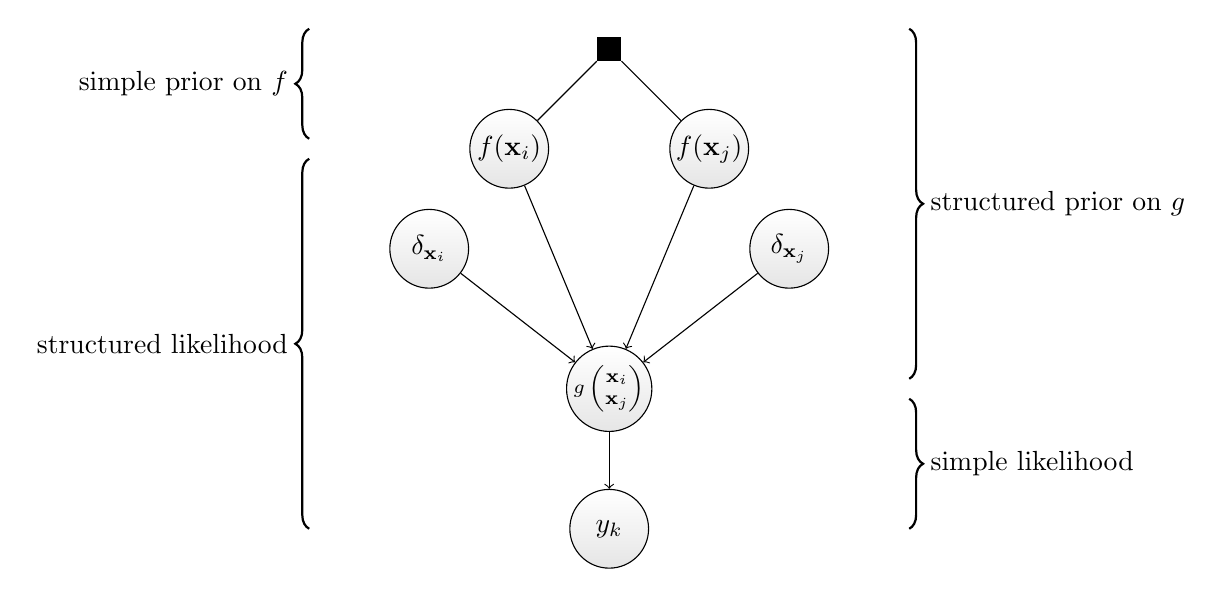
\begin{tikzpicture}
				\node at (2.5in,2.4in) [fill =black, rectangle,inner sep=0pt, minimum size = 0.3cm] (factor) {};
				\node at (2in,1.9in) [draw, circle,inner sep=0pt, minimum size = 1cm, top color=white, bottom color=black!10] (f_1) {$f(\x_i)$};
				\node at (3in,1.9in) [draw, circle,inner sep=0pt, minimum size = 1cm, top color=white, bottom color=black!10] (f_2) {$f(\x_j)$};
				\node at (1.6in,1.4in) [draw, circle,inner sep=0pt, minimum size = 1cm, top color=white, bottom color=black!10] (delta_2) {$\delta_{\x_i}$};	
				\node at (3.4in,1.4in) [draw, circle,inner sep=0pt, minimum size = 1cm, top color=white, bottom color=black!10] (delta_1) {$\delta_{\x_j}$};
				\node at (2.5in,0.7in) [draw, circle,inner sep=0pt, minimum size = 1cm, top color=white, bottom color=black!10] (g) {\scriptsize $g\left(\begin{matrix}\x_i\\\x_j\\\end{matrix}\right)$};
				\node at (2.5in,0in) [draw, circle,inner sep=0pt, minimum size = 1cm, top color=white, bottom color=black!10] (y) {$y_k$};
				\draw [->] (g) to (y);
				\draw  (factor) to (f_1);
				\draw (factor) to (f_2);
				\draw [->] (f_1) to (g);			
				\draw [->] (f_2) to (g);
				\draw [->] (delta_1) to (g);
				\draw [->] (delta_2) to (g);
				\draw [thick,decorate,decoration={brace,amplitude=5pt},] (1in,1.95in)  -- (1in,2.5in)
					node [black,midway,left=4pt] {simple prior on $f$};
				\draw [thick,decorate,decoration={brace,amplitude=5pt}] (1in,0in)  -- (1in,1.85in)
					node [black,midway,left=4pt] {structured likelihood};
				\draw [thick,decorate,decoration={brace,amplitude=5pt}] (4in,2.5in)  -- (4in,0.75in)
									node [black,midway,right=4pt] {structured prior on $g$};
				\draw [thick,decorate,decoration={brace,amplitude=5pt}] (4in,0.65in)  -- (4in,0in)
					node [black,midway,right=4pt] {simple likelihood};
			\end{tikzpicture}
	\end{center}
		\caption{Generative model underlying the preference learning framework. \emph{Left:} the original approach \citep{chu2005} considers the latent preference function $f$ as latent parameter, and the rest of the graphical model as a complex, structured likelihood. \emph{Right:} Our approach re-parametrises the problem in terms of $g$, and thus works with a simpler likelihood but with a more structured prior. The prior takes the form of a Gaussian Process with the preference judgement covariance function. \label{fig:graphical_model}}
\end{figure}


It is straightforward to show that the preference kernel, $k_{pref}$ is positive semi-definite. We can also see how $k_{pref}$ respects the anti-symmetry properties of preference learning, by computing the prior correlation between $g(\x_i,\x_j)$ and $g(\x_j,\x_i)$ as follows (assuming for brevity that $\mu_{pref}=0$):
 
 \begin{align}
 	\text{Corr}&(g(\x_i,\x_j),g(\x_j,\x_i)) = \frac{k_{pref}((\x_i,\x_j),(\x_j,\x_i))}{\sqrt{k_{pref}((\x_i,\x_j),(\x_i,\x_j))}\sqrt{k_{pref}((\x_j,\x_i),(\x_j,\x_i))}} \notag\\
 		&= \frac{k(\x_i,\x_j) + k(\x_j,\x_i) - k(\x_i,\x_i) - k(\x_j,\x_j)}{\sqrt{k(\x_i,\x_i) + k(\x_j,\x_j) - k(\x_i,\x_j) - k(\x_j,\x_i)}\sqrt{k(\x_j,\x_j) + k(\x_i,\x_i) - k(\x_j,\x_i) - k(\x_i,\x_j)}}\notag\\ &= -1\,.\notag
 \end{align}

That is, the value at $(\x_i,\x_j)$ is perfectly anti-correlated with the value at $(\x_j,\x_i)$ under the prior. From this fact it can be shown that all elements $g$ of the reproducing kernel Hilbert space (RKHS) corresponding to $k_{pref}$ have the property that $g(\x_i,\x_j) = -g(\x_j,\x_i)$. 

In summary, the combination of the likelihood in (\ref{eq:likelihood2})
with a GP prior based on this new preference kernel allows us
to transform the problem of learning preferences into a
GP binary classification problem on the space of features
$\mathcal{X}^2$. 
This means that state-of-the art methods
for GP binary classification, such as expectation propagation,
can be trivially used for addressing pairwise preference learning problems.
Furthermore, the simplified likelihood (\ref{eq:likelihood2})
allows us to easily implement complex methods 
such as the following multi-user approach.



\section{A Multi-User Model for Preference Learning \label{sec:model}}

Consider $I$ items with feature vectors $\mathbf{x}_i\in\mathcal{X}$ for $i=1,\ldots,I$. 
The single-user learning approach assumes an independent latent function for the $u$-th user,
$g_u:\mathcal{X}^2\mapsto\mathbb{R}$. Our approach to the multi-user problem is to assume common structure
in the user latent functions. In particular, we assume a set of $D$ shared latent functions,
$h_d:\mathcal{X}^2\mapsto \mathbb{R}$ for $d=1,\ldots,D$, such that the user latent functions are 
generated by a linear combination of these functions, namely

\begin{equation}
g_{u}(\mathbf{x}_j,\mathbf{x}_k)=\sum_{d=1}^{D}w_{u,d}h_{d}(\mathbf{x}_j,\mathbf{x}_k)\,,\label{eq:expressionG}
\end{equation}

here $w_{u,d}\in \mathbb{R}$ is the weight given to function $h_d$ for user $u$.
We place a GP prior over the shared latent functions $h_{1},\ldots,h_{D}$ using the
preference kernel described in the previous section.
This model allows the preferences of the different users to share
some common structure represented by the latent functions $h_{1},\ldots,h_{D}$.
This approach is similar to unsupervised dimensionality reduction methods that are commonly used for addressing collaborative filtering problems \cite{stern2009,raiko2007}.

We may extend this model further to the case in which, for each user $u$, there is
a feature vector $\mathbf{u}_u \in \mathcal{U}$ containing information that might be useful for prediction.
We denote by $\mathbf{U}$ the set of all the users' feature vectors,
that is, $\mathbf{U} = \{\mathbf{u}_1,\ldots,\mathbf{u}_U\}$.
The user features are incorporated now by placing a separate GP prior over the users weights.
In particular, we replace the scalars $w_{u,d}$ in (\ref{eq:expressionG}) with functions
$w_d'(\mathbf{u}_u):\mathcal{U}\rightarrow\mathcal{\mathbb{R}}$. 
These weight functions describe the contribution of shared latent function
$h_d$ to the user latent function $g_u$ as a function of the user feature vector $\mathbf{u}_u$.

In the multi-user setting we are given a list
$\List=\{p_1,\ldots,p_P\}$ with all the \emph{pairs} of items evaluated by the users, where $P\leq I(I-1)/2$ (the maximum number of pairs).
The data consists of $\List$, the sets of feature vectors for the users $\mathbf{U}$ (if available)
and the items $\mathbf{X}=\{\mathbf{x}_1,\ldots,\mathbf{x}_I\}$, and $U$ different sets of preference judgements,
one for each user, $\mathcal{D}=\{\{z_{u,i},y_{u,i}\}_{i=1}^{M_u}\}_{u=1}^{U}$, where $z_{u,i}$ indexes the $i$-th
pair evaluated by user $u$, $y_{i,u}=1$ if this user
prefers the first item in the pair to the second and $y_{i,u}=-1$ otherwise. $M_u$ is the number of 
preference judgements made by the $u$-th user.

\subsection{Probabilistic Description}

The task of interest is to predict preference on unseen item pairs for a particular user.
To do this we cast the model described above into a probabilistic framework.
Let $\mathbf{G}$ be an $U\times P$ `user-function' matrix, where each row corresponds to
a particular user's latent function, that is, the entry in the $u$-th column and $i$-th row is 
$g_{u,i}= g_u(\mathbf{x}_{\alpha(i)},\mathbf{x}_{\beta(i)})$
and $\alpha(i)$ and $\beta(i)$ denote respectively the first and second item in the $i$-th pair from $\mathcal{L}$.
Let $\mathbf{H}$ be a $D\times P$ `shared-function' matrix,
where each row represents the shared latent functions, that is, the entry in the $d$-th row and $i$-th column is 
$h_{d,i}= h_d(\mathbf{x}_{\alpha(i)},\mathbf{x}_{\beta(i)})$.
Finally, we introduce the $U \times D$ weight matrix $\mathbf{W}$ such that each row contains a user's weights, that is, the entry in the $u$-th row and $d$-th column of this matrix is $w_d'(\mathbf{u}_u)$.
Note that $\mathbf{G} = \mathbf{W} \mathbf{H}$ represents equation (\ref{eq:expressionG}) in matrix form.
Let $\mathbf{T}$ be the $U\times P$ target matrix given by $\mathbf{T} = \text{sign}[\mathbf{G} + \mathbf{E}]$,
where $\mathbf{E}$ is an $U \times P$ noise matrix whose entries are sampled i.i.d. from a standard Gaussian distribution and
the function ``$\text{sign}$'' retains only the sign of the elements in a matrix. 
The observations $y_{u,i}$ in $\mathcal{D}=\{\{z_{u,i},y_{u,i}\}_{i=1}^{M_u}\}_{u=1}^{U}$ are
mapped to the corresponding entries of $\mathbf{T}$ using $t_{u,z_{u,i}} = y_{u,i}$.
Let $\mathbf{T}^{(\mathcal{D})}$ and $\mathbf{G}^{(\mathcal{D})}$ represent the elements of $\mathbf{T}$ and $\mathbf{G}$
corresponding only to the available observations $y_{u,i}$ in $\mathcal{D}$.
Then, the likelihood for $\mathbf{G}^{(\mathcal{D})}$ given $\mathbf{T}^{(\mathcal{D})}$ and conditional distribution for $\mathbf{G}^{(\mathcal{D})}$ given $\mathbf{H}$ and $\mathbf{W}$ are

\begin{align*}
\mathcal{P}(\mathbf{T}^{(\mathcal{D})}|\mathbf{G}^{(\mathcal{D})}) 
= \prod_{u=1}^U \prod_{i=1}^{M_u} \Phi[t_{u,z_{u,i}} g_{u,z_{u,i}}]\,\,\,\text{and}\,\,\,
\mathcal{P}(\mathbf{G}^{(\mathcal{D})}|\mathbf{W},\mathbf{H}) = 
\prod_{u=1}^{U} \prod_{i=1}^{M_u}\delta[g_{u,z_{u,i}}-\mathbf{w}_u\mathbf{h}_{\cdot,z_{u,i}}]\,
\end{align*}

respectively, where $\mathbf{w}_u$ is the $u$-th row in $\mathbf{W}$, $\mathbf{h}_{\cdot,i}$ is the $i$-th column in $\mathbf{H}$
and $\delta$ represents a point probability mass at zero.
We now select the priors for $\mathbf{W}$ and $\mathbf{H}$. 
We assume that each function $w_1',\ldots,w_D'$ is sampled \textit{a priori} from a GP
with zero mean and specific covariance function. Let $\mathbf{K}_\text{users}$ be the $U \times U$ 
covariance matrix for entries in each column of matrix $\mathbf{W}$. Then

\begin{equation}
\mathcal{P}(\mathbf{W}|\mathbf{U})=  
\prod_{d=1}^D \mathcal{N}(\mathbf{w}_{\cdot,d}|\mathbf{0},\mathbf{K}_\text{users})\,,\label{eq:priorW}
\end{equation}

where $\mathbf{w}_{\cdot,d}$ is the $d$-th column in $\mathbf{W}$.
If user features are unavailable, $\mathbf{K}_\text{users}$ becomes the identity matrix.
Finally, we assume that each shared latent function $h_1,\ldots,h_D$ is sampled \textit{a priori} from a GP
with zero mean and covariance function given by a preference kernel. 
Let $\mathbf{K}_\text{items}$ be the $P \times P$ preference covariance 
matrix for the item pairs in $\List$. The prior for $\mathbf{H}$ is then 

\begin{equation}
\mathcal{P}(\mathbf{H}|\mathbf{X},\List) = 
\prod_{j=1}^{D}\mathcal{N}(\mathbf{h}_j|\mathbf{0},\mathbf{K}_\text{items})\,,\label{eq:priorH}
\end{equation}

where $\mathbf{h}_j$ is the $j$-th row in $\mathbf{H}$. The resulting posterior for $\mathbf{W}$, $\mathbf{H}$ and $\mathbf{G}^{(\mathcal{D})}$ is

\begin{equation}
\mathcal{P}(\mathbf{W},\mathbf{H},\mathbf{G}^{(\mathcal{D})}|\mathbf{T}^{(\mathcal{D})},\mathbf{X},\List) =
\frac{\mathcal{P}(\mathbf{T}^{(\mathcal{D})}|\mathbf{G}^{(\mathcal{D})})
\mathcal{P}(\mathbf{G}^{(\mathcal{D})}|\mathbf{W},\mathbf{H})\mathcal{P}(\mathbf{W}|\mathbf{U})\mathcal{P}
(\mathbf{H}|\mathbf{X},\List)}{\mathcal{P}(\mathbf{T}^{(\mathcal{D}}|\mathbf{X},\List)}\,.\label{eq:post}
\end{equation}

Given a new item pair $p_{P+1}$, we can compute the predictive distribution for the preference of the $u$-th user ($1 \leq u \leq U$) on this pair by integrating out the parameters $\mathbf{H},\mathbf{W}$ and $\mathbf{G}^{(\mathcal{D})}$ as follows:

\begin{align}
\mathcal{P}(t_{u,P+1}|&\mathbf{T}^{(\mathcal{D})},\mathbf{X},\List,p_{P+1}) =
\int \mathcal{P}(t_{u,P+1}|g_{u,P+1}) \mathcal{P}(g_{u,P+1}|\mathbf{w}_u,\mathbf{h}_{\cdot,P+1})\notag\\
 & \quad \mathcal{P}(\mathbf{h}_{\cdot,P+1}|\mathbf{H},\mathbf{X},\List,p_{P+1})
\mathcal{P}(\mathbf{H},\mathbf{W},\mathbf{G}^{(\mathcal{D})}|\mathbf{T}^{(\mathcal{D})},\mathbf{X},\List)
\,d\mathbf{H}\,d\mathbf{W}\,d\mathbf{G}^{(\mathcal{D})}\,,
\label{eq:predictions}
\end{align}
where $\mathcal{P}(t_{u,P+1}|g_{u,P+1})=\Phi[t_{u,P+1}g_{u,P+1}]$,
$\mathcal{P}(g_{u,P+1}|\mathbf{w}_u,\mathbf{h}_{\cdot,P+1})=\delta[ g_{u,P+1} - \mathbf{w}_u \mathbf{h}_{\cdot,P+1}]$,
\begin{equation}
\mathcal{P}(\mathbf{h}_{\cdot,P+1}|\mathbf{H},\mathbf{X},\List,p_{P+1})
=\prod_{d=1}^D \mathcal{N}(h_{d,P+1}|\mathbf{k}_\star^\text{T} \mathbf{K}^{-1}_\text{items} \mathbf{h}_d, k_\star -
\mathbf{k}_\star^\text{T}  \mathbf{K}^{-1}_\text{items} \mathbf{k}_\star)
\label{eq:predictive}
\end{equation}
$k_\star$ is the prior variance of $h_d(\mathbf{x}_{\alpha(P+1)}, \mathbf{x}_{\beta(P+1)})$
and $\mathbf{k}_\star$ is a $P$-dimensional vector that contains the prior covariances between $h_d(\mathbf{x}_{\alpha(P+1)}, \mathbf{x}_{\beta(P+1)})$
and $h_d(\mathbf{x}_{\alpha(1)}, \mathbf{x}_{\beta(1)}),\ldots,h_d(\mathbf{x}_{\alpha(P)}, \mathbf{x}_{\beta(P)})$.

In practice, computing (\ref{eq:post}) or (\ref{eq:predictive})
is infeasible and approximate inference has to be used.
For this task, we propose to use a combination of expectation propagation (EP) \cite{Minka2001} and variation Bayes (VB) \cite{Attias1999}.
Empirical studies show that EP obtains state-of-the-art performance 
in the related problem of GP binary classification \cite{nickisch2008}.

Typically, data with which to learn the model is limited, and furthermore the computational 
time required to train and make predictions can become large when the volume of data becomes very large (there is further discussion of computational complexity in Sections \ref{sec:sparse} and \ref{sec:relatedWork}).  
Therefore, we want to learn about the users' preferences with the proposed model
using the least amount of data possible, or equivalently, extract maximal useful information from a 
limited number of observations. Therefore we query
users actively about their preferences on the most informative pairs of items \cite{brochu2007}.
Next, we describe a novel method to implement this strategy.
This method exploits the preference kernel and so may
be trivially generalized to GP binary classification problems also.

\section{Bayesian active learning by disagreement\label{sec:active}}

The goal of active learning is to choose item pairs such that we learn the
preference functions for the users using minimal data.
Information theoretic approaches to active learning are popular because
they do not require prior knowledge of loss functions or test domains.
The central goal is to identify the new data point that maximizes the expected reduction in
posterior entropy. For preference learning
(see Section \ref{sec:prefKernel}), this implies
choosing the new item features $\mathbf{x}_i$ and $\mathbf{x}_j$ that maximize

\vspace{-0.65cm}
{\small
\begin{align}   
\ent[\mathcal{P}(g|\mathcal{D})] - \E_{\mathcal{P}(y|\mathbf{x}_i,\mathbf{x}_j,\data)} \left[ \ent[\mathcal{P}(g|y,\mathbf{x}_i,\mathbf{x}_j,\data)]\right]\,,
\label{eqn:ent_change}
\end{align}
}

\vspace{-0.65cm}
\normalsize where $\mathcal{D}$ are the user preferences observed so far and
$\ent[p(x)]=-\int p(x)\log p(x)\,dx$ represents the Shannon entropy. 
This framework, originally proposed in \cite{lindley1956},
is difficult to apply directly to models based on GPs.
In these models, entropies can be poorly
defined or their computation can be intractable.
In practice, current approaches make
approximations for the computation of the posterior entropy \cite{mackay1992,lawrence2002}. 
However, a second difficulty arises; if $n$ new data points are
available for selection, with $|\{-1,1\}|=2$ possible values for $y$.
Then $\mathcal{O}(2n)$ potentially expensive posterior updates are required to find the maximizer
of (\ref{eqn:ent_change}): one for every available feature vector and possible class value.
This is often too expensive in practice.

A solution consists in noting that (\ref{eqn:ent_change}) is equivalent to the conditioned mutual information between $y$ and $g$.
Using this we can rearrange this equation to compute entropies in $\y$ space:

\vspace{-0.65cm}
{\small
\begin{align}
\ent[\mathcal{P}(y|\mathbf{x}_i,\mathbf{x}_j,\data)] - \E_{\mathcal{P}(g|\data)}
\left[\ent\left[ \mathcal{P}(y|\mathbf{x}_i,\mathbf{x}_j,g)\right]\right]\,. \label{eqn:rearrangement} 
\end{align}
}

\vspace{-0.65cm}
\normalsize This overcomes the previous challenges. Entropies are now evaluated in
output space, which has low dimension. Furthermore, $g$ is now conditioned only upon $\data$,
so only $\mathcal{O}(1)$ updates of the posterior distribution are required. 
We only need to recompute the posterior once per data point selected, not for every possible data point under consideration.
Expression (\ref{eqn:rearrangement}) also provides us with an intuition about the objective;
we seek the $\mathbf{x}_i$ and $\mathbf{x}_j$ for which a) the model is marginally
uncertain about $y$ (high $\ent[\mathcal{P}(\y | \mathbf{x}_i,\mathbf{x}_j, \data)]$) and
b) conditioned on a particular value of $g$ the model is confident about $y$
(low $\E_{\mathcal{P}(g|\data)} \left[\ent [ \mathcal{P}(y |\mathbf{x}_i,\mathbf{x}_j,g] \right)]$).
This can be interpreted as seeking the pair $\mathbf{x}_i$ and $\mathbf{x}_j$ for which the latent functions $g$, under the posterior, `disagree' with each other the most about the outcome, that is, the preference judgement.
Therefore, we refer to this objective as Bayesian Active Learning by Disagreement (BALD).
This method is independent of the approach used for inference, something which does not hold for
the techniques described in \cite{mackay1992, krishnapuram2004, lawrence2002}. 
In the following section we show how (\ref{eqn:rearrangement}) can be applied to binary classification with GPs, and hence via the preference kernel also to any preference learning problem.


\subsection{BALD in binary classification with GPs}

\begin{SCfigure}
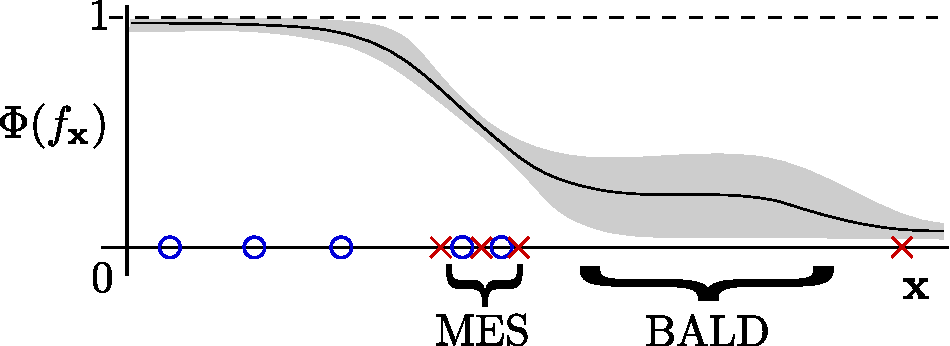
\includegraphics[scale = 0.45]{figs/BALD_eg.pdf}
\caption{Toy example with 1D input. Circles and crosses
denote labelled data. The plot shows the mean and variance of the GP predictive
distribution. Maximum Entropy Sampling (MES)
samples from the region of highest marginal uncertainty, ignoring the
second term in \eqref{eqn:rearrangement}. BALD samples 
from the region of greatest uncertainty in the latent function.\label{fig:BALD}}
\end{SCfigure}

Most approximate inference methods for the problem of binary classification with
GPs produce a Gaussian approximation to the posterior distribution of $f$, the
latent function of interest. In the binary GP classifier, the entropy of $y$ given the corresponding value of $f$ 
can be expressed in terms of the binary entropy function, $\mathrm{h}[f]=- f\log f - (1-f)\log(1-f)$.
In particular,
$\ent[p(y\vert\x,\latfun)] = \mathrm{h}\left[\Phi(\latfun(\x)\right]$.
When a Gaussian is used to approximate the posterior of $f$,  we have that
for each $\x$, $\latfun_{\x} = \latfun(\x)$ will follow a Gaussian distribution with mean $\mu_{\x}$ and
variance $\sigma_{\x}^2$.
The first term in (\ref{eqn:rearrangement}), that is, $\ent[p(y\vert\x,\data)]$, can be handled analytically in this case:
$\ent[p(y\vert\x,\data)] \approx \mathrm{h}\left[ \int \Phi( \latfun_{\x} )
\mathcal{N}(\latfun_{\x}| \mu_{\x},\sigma_{\x}^2) d\latfun_{\x} \right]
= \mathrm{h} \left[ \Phi\left( \mu_{\x} (\sigma^2_{\x} + 1)^{-1/2}\right)\right]$,
where $\approx$ represents here the Gaussian approximation to the posterior of $\latfun_{\x}$.
The second term in (\ref{eqn:rearrangement}), that is,
$\E_{p(\latfun\vert\data)} \left[ \ent[p(\y\vert\x, \latfun)] \right]$, can be approximated as
$ \E_{p(f\vert\data)} \left[ \ent[p(\y\vert\x, \latfun)] \right] \approx
C(\sigma_{\x}^2 + C^2)^{-1/2}\exp\left(-\mu_{\x}^2(2\left(\sigma_{\x}^2 + C^2\right))^{-1}\right)$,
where $C=\sqrt{\pi\log 2 / 2}$. This result is obtained by
using the Gaussian approximation to the posterior of $\latfun_{\x}$
and then approximating $\mathrm{h}[\Phi(\latfun_{\x})]$
by the squared exponential curve $\exp(-\latfun_{\x}^2/\pi\log 2)$
(details can be found in Section 3 of the supplementary material).

To summarize, the BALD algorithm for active binary GP classification / preference learning first applies
any approximate inference method to obtain the posterior mean
$\mu_{\x}$ and variance $\sigma_{\x}^2$ of $f$ at each point of interest $\x$. Then, it selects the
feature vector $\x$ that maximizes the objective

\vspace{-0.5cm}
{\small
\begin{equation}
\mathrm{h} \left[ \Phi\left( \mu_{\x}(\sigma^2_{\x} + 1)^{-1/2} \right)\right] -
C(\sigma_{\x}^2 + C^2)^{-1/2} \exp\left(-\mu_{\x}^2(2\left(\sigma_{\x}^2 + C^2\right))^{-1}\right)\,.\label{eqn:BALD}
\end{equation}
}

\vspace{-0.6cm}
\normalsize BALD assigns a high value to the feature vector $\x$ when the model is both uncertain
about the label ($\mu_{\x}$ close to 0) and there is high uncertainty about $f_\x$
($\sigma_{\x}^2$ is large). The second term prevents BALD from sampling in regions
where the model knows that the label is uncertain. Figure \ref{fig:BALD} illustrates
the differences between BALD and Maximum Entropy Sampling \cite{sebastiani2000} (details in the supplementary material, Section 5).
MES considers only marginal uncertainty (the first term in \eqref{eqn:BALD}), and hence seeks data in an
uninformative region of the plot. By contrast, BALD samples data from the
region of greatest uncertainty in the latent function.

\section{Expectation Propagation and Variational Bayes\label{sec:ep}}

This proposed method for approximate inference in our multi-user model is based on the combination of expectation propagation \cite{Minka2002,gerven2010a}
and variational inference \cite{stern2009}. We first describe the general version of the algorithm.
Finally, in Section \ref{sec:sparse}, we describe the version which employs sparse approximations to the covariance matrices $\mathbf{K}_\text{users}$
and $\mathbf{K}_\text{items}$ for speeding up computations.

The proposed EP method approximates the exact posterior distribution by the following parametric distribution:

\begin{eqnarray}
\mathcal{Q}(\mathbf{G}^{(\mathcal{D})},\mathbf{W},\mathbf{H}) & = & \left[\prod_{u=1}^{U}\prod_{d=1}^{D}\mathcal{N}(w_{ud}|m_{u,d}^{w},v_{u,d}^{w})\right]
\left[\prod_{d=1}^{D}\prod_{i=1}^{P} \mathcal{N}(h_{d,i}|m_{d,i}^h,v_{d,i}^{h})\right]\nonumber\\
& & \left[\prod_{u=1}^N \prod_{j=1}^{M_u} \mathcal{N}(g_{u,z_{u,j}}|m_{u,j}^g,v_{u,j}^g)\right]\,,\label{eq:epPostApprox}
\end{eqnarray}

where $m_{u,d}^w$, $v_{u,d}^w$, $m_{d,i}^h$, $v_{d,i}^h$,
$m_{u,j}^g$, and $v_{u,j}^g$ are free parameters to be determined by EP. 
The joint distribution of the model parameters and the data 
$\mathcal{P}(\mathbf{G}^{(\mathcal{D})},\mathbf{W},\mathbf{H},\mathbf{T}^{(\mathcal{D})},\mathbf{X},\ell)$ can be factorized
into four factors $f_1,\ldots,f_4$, namely,

\begin{equation}
\mathcal{P}(\mathbf{G}^{(\mathcal{D})},\mathbf{W},\mathbf{H},\mathbf{T}^{(\mathcal{D})},\mathbf{X},\ell) =
\prod_{k=1}^4 f_a(\mathbf{G}^{(\mathcal{D})},\mathbf{W},\mathbf{H})\,,
\end{equation}

where $f_1(\mathbf{G}^{(\mathcal{D})},\mathbf{W},\mathbf{H}) = \mathcal{P}(\mathbf{T}^{(\mathcal{D})}|\mathbf{G}^{(\mathcal{D})})$,
$f_2(\mathbf{G}^{(\mathcal{D})},\mathbf{W},\mathbf{H}) = \mathcal{P}(\mathbf{G}^{(\mathcal{D})}|\mathbf{W},\mathbf{H})$,
$f_3(\mathbf{G}^{(\mathcal{D})},\mathbf{W},\mathbf{H}) = \mathcal{P}(\mathbf{W}|\mathbf{U})$ and
$f_4(\mathbf{G}^{(\mathcal{D})},\mathbf{W},\mathbf{H}) = \mathcal{P}(\mathbf{H}|\mathbf{X},\ell)$.
EP approximates each of these exact factors by 
approximate factors $\hat{f}_{1}(\mathbf{W},\mathbf{H},\mathbf{G}^{(\mathcal{D})}),\ldots,\hat{f}_{4}(\mathbf{W},\mathbf{H},\mathbf{G}^{(\mathcal{D})})$
that have the same functional form as (\ref{eq:epPostApprox}), namely,

\begin{eqnarray}
\hat{f}_a(\mathbf{G}^{(\mathcal{D})},\mathbf{W},\mathbf{H}) & = &
\left[\prod_{u=1}^{U}\prod_{d=1}^{D}\mathcal{N}(w_{ud}|\hat{m}_{u,d}^{a,w},\hat{v}_{u,d}^{a,w})\right]
\left[\prod_{d=1}^{D}\prod_{i=1}^{P} \mathcal{N}(h_{d,i}|\hat{m}_{d,i}^{a,h},\hat{v}_{d,i}^{a,h})\right]\nonumber\\
& & \left[\prod_{u=1}^N \prod_{j=1}^{M_u} \mathcal{N}(g_{u,z_{u,j}}|\hat{m}_{u,j}^{a,g},\hat{v}_{u,j}^{a,g})\right] \hat{s}_a\,,
\end{eqnarray}

where $a=1,\ldots,4$ and $\hat{m}_{u,d}^{a,w}$, $\hat{v}_{u,d}^{a,w}$, $\hat{m}_{d,i}^{a,h}$, $\hat{v}_{d,i}^{a,h}$,
$\hat{m}_{u,j}^{a,g}$, $\hat{v}_{u,j}^{a,g}$ and $\hat{s}_a$ are free parameters to be determined by EP. 
The posterior approximation $\mathcal{Q}(\mathbf{w},\mathbf{H},\mathbf{G}^{(\mathcal{D})})$
is obtained as the normalized product of the approximate factors $\hat{f}_{1},\ldots,\hat{f}_{4}$, that is,

\begin{equation}
\mathcal{Q}(\mathbf{W},\mathbf{H},\mathbf{G}^{(\mathcal{D})}) \propto
\hat{f}_{1}(\mathbf{W},\mathbf{H},\mathbf{G}^{(\mathcal{D})})\cdots\hat{f}_{4}(\mathbf{W},\mathbf{H},\mathbf{G}^{(\mathcal{D})})\,.
\end{equation}

The first step of EP is to initialize all the approximate factors $\hat{f}_1,\ldots,\hat{f}_4$ and the posterior approximation $\mathcal{Q}$ to be uniform.
In particular,
$m_{u,d}^w=m_{d,i}^h=m_{u,j}^g=\hat{m}_{u,d}^{w,a}=\hat{m}_{d,i}^{a,h}=\hat{m}_{u,j}^{g,a}=0$ and 
$v_{u,d}^w = v_{d,i}^h = v_{u,j}^g = \hat{v}_{u,d}^{a,w} = \hat{v}_{d,i}^{a,h} = \hat{v}_{u,j}^{a,h} = \infty$ for
$a=1,\ldots,4$, $u=1,\ldots,U$, $d=1,\ldots,D$, $i=1,\ldots,P$ and $j = 1,\ldots,M_u$.
After that, EP refines the parameters of the approximate factors by iteratively minimizing the Kullback-Leibler (KL) divergence
between $\mathcal{Q}^{\setminus a}(\mathbf{W},\mathbf{H},\mathbf{G}^{(\mathcal{D})})f_a(\mathbf{W},\mathbf{H},\mathbf{G}^{(\mathcal{D})})$
and $\mathcal{Q}^{\setminus a}(\mathbf{W},\mathbf{H},\mathbf{G}^{(\mathcal{D})})\hat{f}_a(\mathbf{W},\mathbf{H},\mathbf{G}^{(\mathcal{D})})$, for $a=1,\ldots,4$,
where $\mathcal{Q}^{\setminus a}$ is the ratio between $\mathcal{Q}$ and $\hat{f}_a$. That is, EP iteratively minimizes

\begin{equation} 
\text{D}_{\text{KL}}(Q^{\setminus a}f_a\|Q^{\setminus a}\hat{f}_a) 
= \int \left[Q^{\setminus a}f_a \log \frac{Q^{\setminus a}f_a}{Q^{\setminus a}\hat{f}_a}+
Q^{\setminus a}\hat{f}_a-Q^{\setminus a}f_a\right]\,d\mathbf{W}\,d\mathbf{H}\,d\mathbf{G}^{(\mathcal{D})}\label{eq:KL}
\end{equation}

with respect to $\hat{f}_a$, for $a = 1,\ldots,4$.
The arguments to $Q^{\setminus a}f_a $ and 
$Q^{\setminus a}\hat{f}_a$ have been omitted in the 
right-hand side of (\ref{eq:KL}) to improve the readability of the expression.
However, the minimization of (\ref{eq:KL}) does not perform well when we have to refine the parameters of $\hat{f}_2$.
The reason for this is that the corresponding exact factor $f_2$ (equation (7) in the main document)
is invariant to simultaneous changes in sign, scalings, or rotations of the entries of $\mathbf{W}$ and $\mathbf{H}$.
This non-identifiability in the latent space spanned by $\mathbf{W}$ and $\mathbf{H}$
originates multiple modes in the distribution $Q^{\setminus 2}f_2$.
The minimization of the direct version of the KL divergence results in an approximation that averages across all
of the modes, leading to poor predictive performance.
We solve this problem by following an approach similar to the one described by \cite{stern2009}.
Instead of minimizing $\text{KL}(\mathcal{Q}^{\setminus 2} f_2 \| \mathcal{Q}^{\setminus 2} \hat{f}_2)$,
we refine $\hat{f}_2$ by minimizing the reversed version of the KL divergence, that is,
we minimize $\text{KL}(\mathcal{Q}^{\setminus 2} \hat{f}_2 \| \mathcal{Q}^{\setminus 2} f_2)$ with respect to the parameters of $\hat{f}_2$.
The reversed version of the divergence has mode seeking properties \citep{Bishop2007} and tends to approximate
only a single mode of the target distribution, leading to better predictive accuracy.

The EP algorithm iteratively refines the approximate factors until convergence.
We assume the algorithm has converged when the absolute value of the change in the parameters
$m_{u,i}^g$ of $\mathcal{Q}$, where $u = 1,\ldots,U$ and $i = 1,\ldots,M_u$,
is less than a threshold $\delta = 10^{-2}$ between two consecutive cycles of EP,
where a cycle consists in the sequential update of all the approximate factors.
However, convergence is not guaranteed and
EP may end up oscillating without ever stopping \citep{Minka2001}.
This undesirable behavior can be prevented by \emph{damping} the EP updates \citep{Minka2002}.
Let $\hat{f}_a^\text{new}$ denote the value of the approximate factor that minimizes the Kullback-Leibler
divergence. Damping consists of using

\begin{equation}
\hat{f}_a^\text{damp} = \left[ \hat{f}_a^\text{new} \right]^\epsilon \left[ \hat{f}_a \right]^{(1 - \epsilon)}\,,\label{eq:damping}
\end{equation}

instead of $\hat{f}_a^\text{new}$ for the update of each approximate factor $a = 1,\ldots,4$.
The quantity $\hat{f}_a$ represents in (\ref{eq:damping})
the factor before the update. The parameter
$\epsilon \in [0,1]$ controls the amount of damping.
The original EP update (that is, without damping)
is recovered in the limit $\epsilon = 1$. For $\epsilon = 0$,
the approximate factor $\hat{f}_a$ is not modified.
To improve the converge of EP, we use a damping scheme
with a parameter $\epsilon$ that is initialized to 1
and then progressively annealed as recommended by \cite{HernandezLobato2010}.
After each iteration of EP, the value of
this parameter is multiplied by a constant $k < 1$.
The value selected for $k$ is $k = 0.95$.
In the experiments performed, EP performs on average about 50 iterations.

\subsection{The EP predictive distribution}

EP can also approximate the predictive distribution, given by equation (11) in the main manuscript. 
For this, we replace the exact posterior with the EP approximation $\mathcal{Q}$. In this way, we obtain

\begin{equation}
\mathcal{P}(t_{u,P+1}|\mathbf{T}^{(\mathcal{D})},\mathbf{X},\ell,p_{P+1}) \approx 
\Phi\left[t_{u,P+1} m_{u,P+1}^g(v_{u,P+1}^g + 1)^{-\frac{1}{2}}\right]\,,
\end{equation}

where

\begin{align}
m_{u,P+1}^g & = \sum_{d=1}^D  m_{u,d}^w m_{d,P+1}^h\,,\\
v_{u,P+1}^g & = \sum_{d=1}^D  [m_{u,d}^w]^2 v_{d,P+1}^h + \sum_{d=1}^D v_{u,d}^w [m_{d,P+1}^h]^2 + \sum_{d=1}^D v_{u,d}^w v_{d,P+1}^h
\end{align}

and $m_{d,P+1}^h$ and $v_{d,P+1}^h$ for $d = 1,\ldots,D$ are given by

\begin{align}
m_{d,P+1}^h & = \mathbf{k}_\star^\text{T} \left[ \mathbf{K}_\text{items} +
\text{diag}[\hat{\mathbf{v}}_d^{h,2}] \right]^{-1} \hat{\mathbf{m}}_d^{h,2}\,,\label{eq:predictiveMean}\\
v_{d,P+1}^h & = k_\star - \mathbf{k}_\star^\text{T} \left[ \mathbf{K}_\text{items} +
\text{diag}[\hat{\mathbf{v}}_d^{h,2}] \right]^{-1} \mathbf{k}_\star\,,\label{eq:predictiveVariance}
\end{align}

where $k_\star$ is the prior variance of $h_d(\mathbf{x}_{\alpha(P+1)}, \mathbf{x}_{\beta(P+1)})$,
$\mathbf{k}_\star$ is a $P$-dimensional vector that contains the prior covariances between $h_d(\mathbf{x}_{\alpha(P+1)}, \mathbf{x}_{\beta(P+1)})$
and $h_d(\mathbf{x}_{\alpha(1)}, \mathbf{x}_{\beta(1)}),\ldots,h_d(\mathbf{x}_{\alpha(P)}, \mathbf{x}_{\beta(P)})$ for $d=1,\ldots,D$,
the function $\text{diag}(\cdot)$ applied to a vector returns a diagonal matrix with that vector in
its diagonal and the vectors $\hat{\mathbf{m}}_d^{h,2}$ and $\hat{\mathbf{v}}_d^{h,2}$ are given by
$\hat{\mathbf{m}}_d^{h,2}=(\hat{m}_{1,d}^{h,2},\ldots,\hat{m}_{P,d}^{h,2})^\text{T}$ and
$\hat{\mathbf{v}}_d^{h,2}=(\hat{v}_{1,d}^{h,2},\ldots,\hat{v}_{P,d}^{h,2})^\text{T}$.

\subsection{The EP update operations}

In this section we describe the EP updates for refining the approximate factors $\hat{f}_1,\ldots,\hat{f}_4$.
For the sake of clarity, we only include the update rules with no damping ($\epsilon = 1$).
Incorporating the effect of damping in these operations is straightforward. 
With damping,  the natural parameters of the approximate factors become 
a convex combination of the natural parameters before and after the 
update with no damping

\begin{align}
[\hat{v}_{u,d}^{w,a}]^{-1}_\text{damp} & = \epsilon [\hat{v}_{u,d}^{w,a}]^{-1}_\text{new}
+ (1 - \epsilon) [\hat{v}_{u,d}^{w,a}]^{-1}_\text{old}\,,\\
[\hat{m}_{u,d}^{w,a}]_\text{damp} [\hat{v}_{u,d}^{w,a}]_\text{damp}^{-1} & =
\epsilon [\hat{m}_{u,d}^{w,a}]_\text{new} [\hat{v}_{u,d}^{w,a}]_\text{new}^{-1} + (1 - \epsilon)
[\hat{m}_{u,d}^{w,a}]_\text{old}[\hat{v}_{u,d}^{w,a}]^{-1}_\text{old}\,,\\
[\hat{v}_{d,i}^{h,a}]^{-1}_\text{damp} & = \epsilon [\hat{v}_{d,i}^{h,a}]^{-1}_\text{new}
+ (1 - \epsilon) [\hat{v}_{d,i}^{h,a}]^{-1}_\text{old}\,,\\
[\hat{m}_{d,i}^{h,a}]_\text{damp} [\hat{v}_{d,i}^{h,a}]_\text{damp}^{-1} & =
\epsilon [\hat{m}_{d,i}^{h,a}]_\text{new} [\hat{v}_{d,i}^{h,a}]_\text{new}^{-1} + (1 - \epsilon)
[\hat{m}_{d,i}^{h,a}]_\text{old}[\hat{v}_{d,i}^{h,a}]^{-1}_\text{old}\,,\\
[\hat{v}_{u,j}^{g,a}]^{-1}_\text{damp} & = \epsilon [\hat{v}_{u,j}^{g,a}]^{-1}_\text{new}
+ (1 - \epsilon) [\hat{v}_{u,j}^{g,a}]^{-1}_\text{old}\,,\\
[\hat{m}_{d,j}^{g,a}]_\text{damp} [\hat{v}_{u,j}^{g,a}]_\text{damp}^{-1} & =
\epsilon [\hat{m}_{u,j}^{g,a}]_\text{new} [\hat{v}_{u,j}^{g,a}]_\text{new}^{-1} + (1 - \epsilon)
[\hat{m}_{u,j}^{g,a}]_\text{old}[\hat{v}_{u,j}^{g,a}]^{-1}_\text{old}\,,
\end{align}

where $u = 1,\ldots,U$, $d = 1,\ldots,D$, $i = 1,\ldots,P$ and $j=1,\ldots,M_u$.
The subscript $\emph{new}$ denotes the value of the parameter 
given by the full EP update operation with no damping.
The subscript $\emph{damp}$ denotes the parameter value given by the
damped update rule. The subscript $\emph{old}$ refers to
the value of the parameter before the EP update.
The updates for the parameters $\hat{s}_1,\ldots,\hat{s}_4$ are not damped. These parameters are initialized to 1 and are only
updated once the EP algorithm has converged.

The factors are refined in the order $\hat{f}_4, \hat{f}_3, \hat{f}_2, \hat{f}_1$ by applying the EP and VB updates described above. Full details of the specific update operations have been relegated to the Supplementary Material.


\subsection{The EP Approximation of the Model Evidence}

The model evidence, or marginal likelihood is given by $\mathcal{P}(\mathbf{T}^{(\mathcal{D})}|\mathbf{X},\ell)$. It is a useful quantity for assessing the quality of the model, and provides a formal tool for selecting hyper-parameters.
Although, like the posterior, it cannot be computed analytically, once EP has converged, we can approximate it using

\begin{align}
\mathcal{P}(\mathbf{T}^{(\mathcal{D})}|\mathbf{X},\ell) \approx \int \prod_{a=1}^4
\hat{f}_a(\mathbf{G}^{(\mathcal{D})},\mathbf{W},\mathbf{H})\,d\mathbf{G}^{(\mathcal{D})}\,d\mathbf{H}\,d\mathbf{W}\,.
\end{align}

The required computations are presented in the Supplementary Material.

Finally, some of the EP updates may generate a negative value for $\hat{v}_{u,i}^{g,a}$, 
$\hat{v}_{u,d}^{w,a}$ or $\hat{v}_{d,j}^{h,a}$, where $u = 1,\ldots,U$, $i = 1,\ldots,M_u$, $j = 1,\ldots,P$ and $i = 1,\ldots,4$.
Negative variances in Gaussian approximate factors 
are common in many EP implementations \citep{Minka2001,Minka2002}.
When this happens, the marginals of the approximate factor with negative 
variances are not density functions. Instead, they
are correction factors that compensate the errors in the corresponding marginals of other approximate factors.
However, these negative variances can lead to failure of the proposed EP algorithm
 - details in the Supplementary Material.
To address this problem, whenever an EP update yields a negative number for any of the
$\hat{v}_{u,i}^{g,a}$, $\hat{v}_{u,d}^{w,a}$ or $\hat{v}_{d,j}^{h,a}$, we do not update this parameter, nor the corresponding
$\hat{m}_{u,i}^{g,a}$, $\hat{m}_{u,d}^{w,a}$ or $\hat{m}_{d,j}^{h,a}$.

\subsection{Sparse Approximations to speed up Computations} \label{sec:sparse}

The computational cost of EP is determined by the operations needed to refine the approximate factors $\hat{f}_3$ and $\hat{f}_4$.
Refinement of $\hat{f}_4$ required inversion of $D$ $P\times P$ matrices, which has cost $\mathcal{O}(DP^3)$. Similarly, for $\hat{f}_3$ we must invert $D$ $U\times U$ matrices, which has cost $\mathcal{O}(DU^3)$.
These costs can be prohibitive when $P$ or $U$ are very large.
Nevertheless, they can be reduced by using sparse approximations to the covariance matrices $\mathbf{K}_\text{users}$
and $\mathbf{K}_\text{items}$. We use the fully independent training conditional or FITC
approximation, also known as the sparse pseudo-input GP (SPGP) \cite{snelson2006}.
With FITC, the $U \times U$ covariance matrix $\mathbf{K}_\text{users}$ is approximated by
$\mathbf{K}_\text{users}' = \mathbf{Q}_\text{users} + \text{diag}(\mathbf{K}_\text{users}-\mathbf{Q}_\text{users})$,
where $\mathbf{Q}_\text{users} = \mathbf{K}_{\text{users},U,U_0} \mathbf{K}_{\text{users},U_0,U_0}^{-1} \mathbf{K}_{\text{users},U,U_0}^\text{T}$.
In this expression, $\mathbf{K}_{\text{users},U_0,U_0}$ is an $U_0 \times U_0$ covariance matrix given by the evaluation
of the covariance function for the users at all possible pairs of $U_0 < U$ locations
or \emph{user pseudo-inputs} $\{\mathbf{u}'_1,\ldots,\mathbf{u}'_{U_0}\}$,
where $\mathbf{u}'_i \in \mathcal{U}$ for $i = 1,\ldots,U_0$, and
$\mathbf{K}_{\text{users},U,U_0}$ is an $U \times U_0$ matrix with the evaluation of
the covariance function for the users at all possible pairs of original user feature vectors and user pseudo-inputs,
that is, $(\mathbf{u}_i, \mathbf{u}_j')$, for $i = 1,\ldots,U$ and $j = 1,\ldots,U_0$.
Similarly, the $P \times P$ covariance matrix $\mathbf{K}_\text{items}$ is also approximated by
$\mathbf{K}_\text{items}' = \mathbf{Q}_\text{items} + \text{diag}(\mathbf{K}_\text{items}-\mathbf{Q}_\text{items})$,
where $\mathbf{Q}_\text{items} = \mathbf{K}_{\text{items},P,P_0} \mathbf{K}_{\text{items},P_0,P_0}^{-1} \mathbf{K}_{\text{items},P,P_0}^\text{T}$,
$\mathbf{K}_{\text{items},P_0,P_0}$ is a $P_0 \times P_0$ covariance matrix given by the evaluation
of the preference kernel at all possible pairs of $P_0 < P$ locations or
\emph{item-pair pseudo-inputs} $\{(\mathbf{x}'_1,\mathbf{x}''_1),\ldots,(\mathbf{x}'_{P_0},\mathbf{x}''_{P_0})\}$,
where $\mathbf{x}'_i,\mathbf{x}''_i \in \mathcal{X}$ for $i = 1,\ldots,P_0$,
and $\mathbf{K}_{\text{items},P,P_0}$ is a $P \times P_0$ matrix with the evaluation of
the preference kernel at all possible combinations of feature vectors for the original item pairs and item-pair pseudo-inputs,
that is, $((\mathbf{x}_{\alpha(i)},\mathbf{x}_{\beta(i)}), (\mathbf{x}'_j,\mathbf{x}''_j))$, for $i = 1,\ldots,P$ and $j = 1,\ldots,P_0$.

Detailed description of how to refine the third and fourth approximate factors when $\mathbf{K}_\text{users}$ and
$\mathbf{K}_\text{items}$ are replaced by $\mathbf{K}_\text{users}'$ and $\mathbf{K}_\text{items}'$, respectively may be found in the Supplementary material.
The required operations are can be efficiently implemented using the formulas
described in \citep{Guzman2007} and \citep{Lazaro2010}.
The resulting complexity of inference, after applying the FITC approximation to update $\hat{f}_3$ and $\hat{f}_4$ is $\mathcal{O}(DU_0^2U)$ and $\mathcal{O}(DP_0^2P)$ operations, respectively.

We now have a flexible multi-user model in which we can perform inference in reasonable computational time. In the following section we will compare our model to two current approached to probabilistic multi-user preference learning, and compare BALD to other popular algorithms for active learning.

\section{Related Methods \label{sec:relatedWork}}

\subsection{Multi-User Preference Learning}

\paragraph{Model of Birlutiu et al.}

As in the single-task preference learning model, a different GP classifier is
fitted to the data generated by each user. However, the different classifiers are now connected by a
common GP prior for the latent preference functions which is optimized to fit the data \cite{birlutiu2009}.
Let $g_u$ be the $u$-th user's latent preference function and let 
$\bm g_u$ be the $k$-dimensional vector with the evaluation of this function at all the observed pairs of items, that is, $k = P$.
Let $\bar{\bm \mu}$ and $\bar{\bm \Sigma}$ denote the prior mean and prior covariance matrix of $\bm g_u$.
Then $\bar{\bm \mu}$ and $\bar{\bm \Sigma}$ are iteratively refined by an EM algorithm which iterates the following steps:
\begin{description}
\item[E-step] Estimate the sufficient statistics (mean $\bm \mu_u$ and covariance matrix $\bm \Sigma_u$) of the posterior distribution of $\bm g_u$
for user $u=1,\ldots,U$, given the current estimates at step $t$ of the parameters $\bar{\bm \mu}^{(t)}$ and $\bar{\bm \Sigma}^{(t)}$ of the
common GP prior.
\item[M-step] Re-estimate the parameters of the GP prior using
\begin{align}
\bar{\bm \mu}^{(t+1)} & = \frac{1}{U} \sum_{u=1}^U \bm \mu_u\,,\nonumber\\
\bar{\bm \Sigma}^{(t+1)} & = \frac{1}{U} \sum_{u=1}^U \bm (\bar{\bm \mu}^{(t)} - \bm \mu_u)^\text{T} (\bar{\bm \mu}^{(t)} - \bm \mu_u) + 
\frac{1}{U}\sum_{u=1}^U \bm \Sigma_u \,.\nonumber
\end{align}
\end{description}
On the first iteration of the EM algorithm we fix $\bar{\bm \mu}^{(0)} = \bm 0$ and compute $\bar{\bm \Sigma}^{(0)}$ 
by evaluating a preference covariance function at all the possible pairs of items. This preference covariance function
is generated by a squared exponential kernel with unit lengthscale. 
The computational cost of the EM algorithm is rather high
since each iteration requires the inversion of $U$ covariance matrices of dimension $P \times P$,
where $P$ is the total number of observed item pairs, is $\mathcal{O}(UP^3)$.
As described in Section \ref{sec:sparse}, the cost of our equivalent algorithm 
(i.e. where we do not incorporate user features) is $\mathcal{O}(DP^3)$, which, even before
including the FITC approximation is significantly cheaper because $D\ll U$.
To reduce the computational burden, we limit
the number of iterations of the EM algorithm to 20. In our experiments, increasing the number of EM iterations 
above 20 did not lead to improvements in the predictive performance of this method.

Birlutiu's approach has an advantage that it learns the full covariance matrix
over the $P$ item pairs for each user, this makes the model flexible,
but causes the poor scalability with the number of users.
We note that the original implementation in \citep{birlutiu2009} does not
use the preference kernel, and used a sampling-based implementation.
We expect that our implementation of this model that uses
the preference kernel
propagation, which is known to perform well with Gaussian processes \citep{nickisch2008},
will augment its performance, but it provides the fairest comparison of 
the underlying model.

\paragraph{Model of Bonilla et al.}

An alternative multi-user model for learning pairwise user preferences is described in \cite{Bonilla2010}.
This approach is based on the assumption that users with similar characteristics or feature vectors should
have similar preferences. In particular, there is a single large latent function $g$ which depends on both
the features of the two items to be compared, $\mathbf{x}_i$ and $\mathbf{x}_j$, and
the specific feature vector for the user who makes the comparison, $\mathbf{u}_u$.
Within the framework of the preference kernel, the likelihood function for Bonilla's model is
\begin{equation}
\mathcal{P}(y|\mathbf{u}_u,\mathbf{x}_i,\mathbf{x}_j,g) = \Phi(yg(\mathbf{x}_i,\mathbf{x}_j,\mathbf{u}_u)
\end{equation}
and the prior for the utility function $g$ is a Gaussian process with zero mean and covariance function 
\begin{equation}
k_\text{Bonilla}((\mathbf{u}_u,\mathbf{x}_i,\mathbf{x}_j), (\mathbf{u}_s,\mathbf{x}_k,\mathbf{x}_l),) =
k_\text{users}(\mathbf{u}_u,\mathbf{u}_s)k_\text{pref}((\mathbf{x}_i,\mathbf{x}_j),(\mathbf{x}_k,\mathbf{x}_l))\,,\label{eq:covBonilla}
\end{equation}
where $k_\text{pref}$ is a preference kernel and $k_\text{users}$ is a covariance function for user features. This latter
function will be large when $\mathbf{u}_u$ and $\mathbf{u}_s$ are similar to each other and small otherwise.
Therefore, the effect of $k_\text{users}$ in (\ref{eq:covBonilla}) is to 
encourage users with similar feature vectors to
agree on their preferences. The preference kernel allows us to do efficient approximate inference in Bonilla's model
using any standard implementation of expectation propagation for the binary classification problem with GPs.
However, the computational cost of Bonilla's method is rather high. 
When the preference kernel is used, the cost of this technique is $\mathcal{O}((\sum_{u=1}^U M_u)^3)$,
where $U$ is the total number of users and $M_u$ is the number of pairs evaluated by the $u$-th user.
By contrast, our approach, when including user features also has complexity $\mathcal{O}(DU^3+DP^3)$. 
In the original work \cite{Bonilla2010} they do not use the preference kernel, this reduces
their complexity to $O((\sum_{u=1}^UI_u)^3)$, where $I_u$ denotes the number of unique items compared
by the $u$-th user. However, this makes inference more complex and they are constrained to using
the Laplace approximation, which is shown to perform less well than EP for with Gaussian Process models \citep{nickisch2008}. Furthermore, this cost is still typically much greater than for our model.
In practice, Bonilla's method is infeasible when
we have observations for more than a few hundred users. Additionally, this method 
requires that feature vectors are available for the different users and that users with similar feature vectors 
generate similar preference observations. When these conditions do not hold, Bonilla's method may
lead to poor predictive performance.
 

\subsection{Active Learning}

\paragraph{Maximum Entropy Sampling} (MES) \citep{sebastiani2000} is similar to BALD in the sense that it also works explicitly in data space
(that is, using equation \eqref{eqn:rearrangement}). MES was proposed for regression models with input-independent observation noise.
In this scenario, the noise in the target variable $y$ does not depend on the input $\mathbf{x}$ and
the second term in equation \eqref{eqn:rearrangement} is constant and can be safely ignored.
However, if noise in the target variable is not input-independent, MES will tend to sample regions of the input space
where uncertainty in $g$ is low but uncertainty in the labels (because of observation noise) is high,
as illustrated in Figure \ref{fig:BALD}.

\paragraph{Query by Committee} (QBC) makes a different approximation to \eqref{eqn:rearrangement} \citep{freund1997}.
QBC samples parameters from the posterior (called committee members). These parameters are then used to perform a deterministic vote on
the outcome of each candidate $\x$. The $\x$ with the most balanced vote is selected for the next active inclusion in the training set.
This objective is termed the `principle of maximal disagreement'. QBC is similar to
BALD when the objective used by BALD is approximated by sampling from the posterior, with the exception
that BALD uses a probabilistic measure of disagreement (equation \eqref{eqn:rearrangement}).
Note that the deterministic vote criterion used by QBC does not take into account
the confidence of the learning method on its predictions. Because of this, QBC can exhibit the same pathologies as MES.

\paragraph{The Informative Vector Machine} (IVM) \citep{lawrence2002} is also motivated by information theory.
This method was originally designed for sub-sampling a dataset and not for addressing online active learning problems.
The IVM requires that the target variables $y$ are observed prior to making a query and it is therefore not applicable online active learning tasks.
Nonetheless, BALD can be applied to the dataset sub-sampling problem for which the IVM is designed, it is simply equipped with less information.
The IVM works with equation \eqref{eqn:ent_change} instead of \eqref{eqn:rearrangement}. Entropies for the latent function $g$ are
calculated approximately in the marginal subspace corresponding to the observed data points.
For this, the IVM employs a Gaussian approximation to the posterior distribution at these locations.
The posterior approximation must be updated to evaluate the entropy decrease after the inclusion
of each candidate data point. If there are $n$ candidate inputs under consideration, a total of $\mathcal{O}(n)$ posterior
updates are required. By contrast, BALD only requires $\mathcal{O}(1)$ updates.
In practice, the IVM approach is infeasible in sophisticated models such as the proposed multi-user approach.

Finally, \cite{tong2001} propose an algorithm for active learning with support vector machines.
This method approximates the version space (the set of hyper-planes consistent with the data)
with a simpler object, such as a hyper-sphere. The algorithm selects the data point whose
dual plane is closest to bisecting this hyper-sphere. 

%\paragraph{Expected Value of Information} Another flavor of approaches is proposed for multi-user preference learning is to use the EVOI \citep{bonilla2010}. This is a decision theoretic approach, and the objective is not to learn optimally about the parameters but to seek the data that is expected to improve the maximum of users latent function the most (i.e. find their most preferred item). This of course requires the set or distribution over test items to be known; although in general this will not be true it is a reasonable assumption for a recommendation application. This approach is well tailored for online active learning with a single user as it seeks to find the best recommendation as fast as possible, whereas the information theoretic approach is more suited when trying to learn the model offline from existing data from many users. By focussing just on areas of high preference one is less likely to discover the true latent functions underlying user behavior, our approach directly tries to reduce uncertainty about these alongside the user-specific parameters (i.e. the weights). Perhaps more importantly to calculate the EVOI new predictive distributions need to be calculated for all possible data points under consideration, again requiring $\mathcal{O}(Q_{\pair}Q_{\y})$ posterior updates; we only require one from that may calculate the score for all candidates, this offers a very large computational saving when the number of possible item pairs is large.

\subsection{Binary Classification Investigation}

We describe an experiment used to to compare BALD to these approaches in the context of binary classification with GPs.
The datasets were divided randomly into pool and test sets.
Each algorithm was initialized with two data points, one from each class, drawn randomly from the pool.
The algorithms select points sequentially, and their classification error was assessed on the test set after each query. The procedure was repeated for several random splits of the data to 
assess statistical significance.
Figure \ref{tab:activeTable} provides a summary of the results. 
BALD can be seen to outperform consistently the alternative algorithms across many datasets. The closest competitor is Maximum Entropy Sampling, which we use as a benchmark active learning algorithm for use with the multi-user preference model in the main paper. 

Table \ref{tab:activeTable} depicts an investigation of BALD's power against the aforementioned algorithms and a non-probabilistic SVM-based active learning algorithm of \citep{tong2001}; this algorithm seeks to reduce the size of `Version Space' maximally fast, which is equivalent to the information theoretic approach but for non-probabilistic models.  

We find that BALD is consistently the best performing algorithm, the closest method is MES, whose performance approaches BALD when the data has very low noise.  
We therefore use MES as our benchmark active learning algorithm for our experiments.

\begin{table}\centering
\resizebox{\textwidth}{!}{
\begin{tabular}{lc@{$\pm$}cc@{$\pm$}cc@{$\pm$}cc@{$\pm$}cc@{$\pm$}cc@{$\pm$}cc@{$\pm$}c}
\hline
{\bf Dataset} & \multicolumn{2}{c}{{\bf BALD}}  & \multicolumn{2}{c}{{\bf Random}} & \multicolumn{2}{c}{{\bf Entropy}} & \multicolumn{2}{c}{{\bf $\mbox{QBC}_{2}$}} & \multicolumn{2}{c}{{\bf $\mbox{QBC}_{100}$}} & \multicolumn{2}{c}{{\bf IVM}} & \multicolumn{2}{c}{{\bf SVM}} \\ 
\hline
austra &  {  $ \bm{18.54} $ } & { $ \bm{ 2.94} $ } & {  $ 44.15 $ } & { $ 12.63 $ } & {  $ 22.46 $ } & { $ 6.20 $ } & {  $ 68.38 $ } & { $ 1.38 $ } & {  $ 29.31 $ } & { $ 5.06 $ } & {  $ 28.46 $ } & { $ 6.58 $ } & {  $ 55.00 $ } & { $ 1.00 $ } \\ 

cancer & {  $ \bm{16.80} $}  & { $ \bm{0.59} $ } & {  $ 22.20 $ } & { $ 1.25 $ } & {  $ 21.10 $ } & { $ 0.48 $ } & {  $ 39.65 $ } & { $ 0.41 $ } & {  $ 18.95 $ } & { $ 1.34 $ } & {  $ 21.35 $ } & { $ 0.50 $ } & {  $ 24.40 $ } & { $ 8.30 $ } \\ 

crabs & {  $ 9.80 $ } & { $ 0.58 $ } & {  $ 11.40 $ } & { $ 1.29 $ } & {  $ \bm{9.20} $ } & { $ \bm{0.49} $ } & {  $ 17.00 $ } & { $ 1.26 $ } & {  $ 10.20 $ } & { $ 0.97 $ } & {  $ 13.60 $ } & { $ 1.86 $ } & {  $ 23.20 $ } & { $ 7.29 $ } \\

letter D v. P & {  $ \bm{45.30} $ } & { $ \bm{1.14} $ } & {  $ 92.10 $ } & { $ 2.41 $ } & {  $ 51.50 $ } & { $ 0.83 $ } & {  $ 48.80 $ } & { $ 1.34 $ } & {  $ 49.10 $ } & { $ 1.38 $ } & {  $ 51.00 $ } & { $ 0.84 $ } & \multicolumn{2}{c}{N/A} \\ 

letter E v. F & {  $ \bm{30.17} $ } & { $ \bm{1.11} $ } & {  $ 71.50 $ } & { $ 17.72 $ } & {  $ 34.33 $ } & { $ 0.42 $ } & {  $ 44.67 $ } & { $ 2.12 $ } & {  $ 30.67 $ } & { $ 1.65 $ } & {  $ 33.00 $ } & { $ 2.27 $ } & \multicolumn{2}{c}{N/A} \\ 

vehicle & {  $ \bm{33.20} $ } & { $ \bm{2.11} $ } & {  $ 75.30 $ } & { $ 7.38 $ } & {  $ 36.60 $ } & { $ 1.74 $ } & {  $ 85.20 $ } & { $ 7.16 $ } & {  $ 35.00 $ } & { $ 1.80 $ } & {  $ 38.20 $ } & { $ 2.00 $ } & {  $ 41.60 $ } & { $ 1.64 $ } \\ 

wine & {  $ \bm{8.80} $ } & { $ \bm{0.37} $ } & {  $ 26.60 $ } & { $ 8.57 $ } & {  $ 10.80 $ } & { $ 1.66 $ } & {  $ 36.40 $ } & { $ 8.36 $ } & {  $ 12.60 $ } & { $ 1.78 $ } & {  $ 20.40 $ } & { $ 9.92 $ } & {  $ 23.80 $ } & { $ 3.48 $ } \\ 

wdbc & {  $ \bm{18.15} $ } & { $ \bm{0.37} $ } & {  $ 47.00 $ } & { $ 1.46 $ } & {  $ 22.55 $ } & { $ 1.05 $ } & {  $ 43.85 $ } & { $ 1.39 $ } & {  $ 23.40 $ } & { $ 1.05 $ } & {  $ 21.40 $ } & { $ 0.85 $ } & {  $ 45.70 $ } & { $ 1.75 $ } \\ 
\hline
\end{tabular}
}
\caption{Performance of BALD and other active learning algorithms on several binary classification datasets from the UCI repository. 
Entries indicate the number of datapoints (plus or minus one standard error of the mean) required to achieve $95\%$ of the predictive performance
achieved by including the entire pool set. Bold typeface indicates the best performing algorithm for each dataset. 
N/A indicates that the corresponding algorithms did not meet the $95\%$ performance level by the end of the simulation.\label{tab:activeTable} }
\end{table}


\section{Experiments}\label{sec:experiments}

\subsection{Datasets}

The performance of our collaborative preference model with the BALD active learning strategy
is evaluated in a series of experiments with simulated and real-world data. The datasets were 
pre-processed as follows.

{\bf Synthetic.} We generated $10$ items with feature vectors $\mathbf{x}_i=(x_{i1},x_{i2})$,
where $x_{i1}$ and $x_{i2}$ are uniformly distributed with zero mean and unit variance, for $i = 1,\ldots,10$.
The user preferences are obtained
using $D=5$ latent functions $h_1,\ldots,h_5$ sampled from a Gaussian process
with zero mean and preference kernel given by a squared exponential kernel with unit length-scale.
The preferences for the $u$-th user are generated according to the sign of
$g_u(\mathbf{x}_i, \mathbf{x}_j) = \sum_{d=1}^5 w_{d}'(\mathbf{u}_u) h_d(\mathbf{x}_i, \mathbf{x}_j) + \epsilon_{ij}$,
where $\epsilon_{ij} \sim \mathcal{N}(0,1)$, the user features $\mathbf{u}_u$ are
generated in the same manner as the feature vectors for the items and the functions $w_{1}',\ldots,w_{D}$
follow the same prior distribution as $h_1,\ldots,h_5'$.

{\bf Jura.} 
This dataset contains concentration measurements for 7 heavy metals in soils of the Swiss Jura region at 359 locations \citep{Atteia1994315,Webster1994}.
We standardized the measurements of each heavy metal to have zero mean and unit standard deviation across the whole dataset.
The standardized measurements are used as utility values to generate preferences for any pair of heavy
metals at each location. Therefore, in this dataset, the locations correspond to users and each heavy metal
represents a different item. To generate the item features, we randomly singled out 20 locations.
The item features are given by the standardized measurements obtained at these locations. 
The user features correspond to the $x$ and $y$ coordinates for the measurements as well as the rock and land type.

{\bf MovieLens.} 
This dataset contains 1 million ratings from 6,000 users on 4,000 movies.
A total of 10 movies were randomly selected from the 50 movies with most ratings.
We also selected those users with at least 7 ratings on these 10 movies.
The remaining missing ratings were estimated using a nearest neighbor method.
The ratings for each user were used as utility values in order to generate preferences for each pair of movies.
The features for each user are gender, age and occupation. The features for each movie are genres
such as \emph{action}, \emph{comedy} or \emph{adventure}.

{\bf Sushi.}
This dataset contains complete rankings given by 5,000 users on $10$ different types of sushi \citep{Kamishima05},
where each sushi includes as features style, major group, minor group, heaviness, consumption
frequency, normalized price and sale frequency. The different users are also represented by
a set of features which include gender, age and geographical/regional information.

{\bf Election.}
This dataset contains the votes obtained by 8 political parties (items) at 650 constituencies (users) in
the 2010 general elections in the UK.
We only kept data for those constituencies with at least votes for more than 6 parties. Missing votes
were estimated using a nearest neighbor method. To generate feature vectors for each item,
we randomly singled out 20 constituencies and used the corresponding votes as features.
The features for each `user' are the corresponding coordinates (latitude and longitude) of the centroid of the constituency on the map.


\subsection{Tuning the kernel lengthscale}

\begin{figure}
\centering
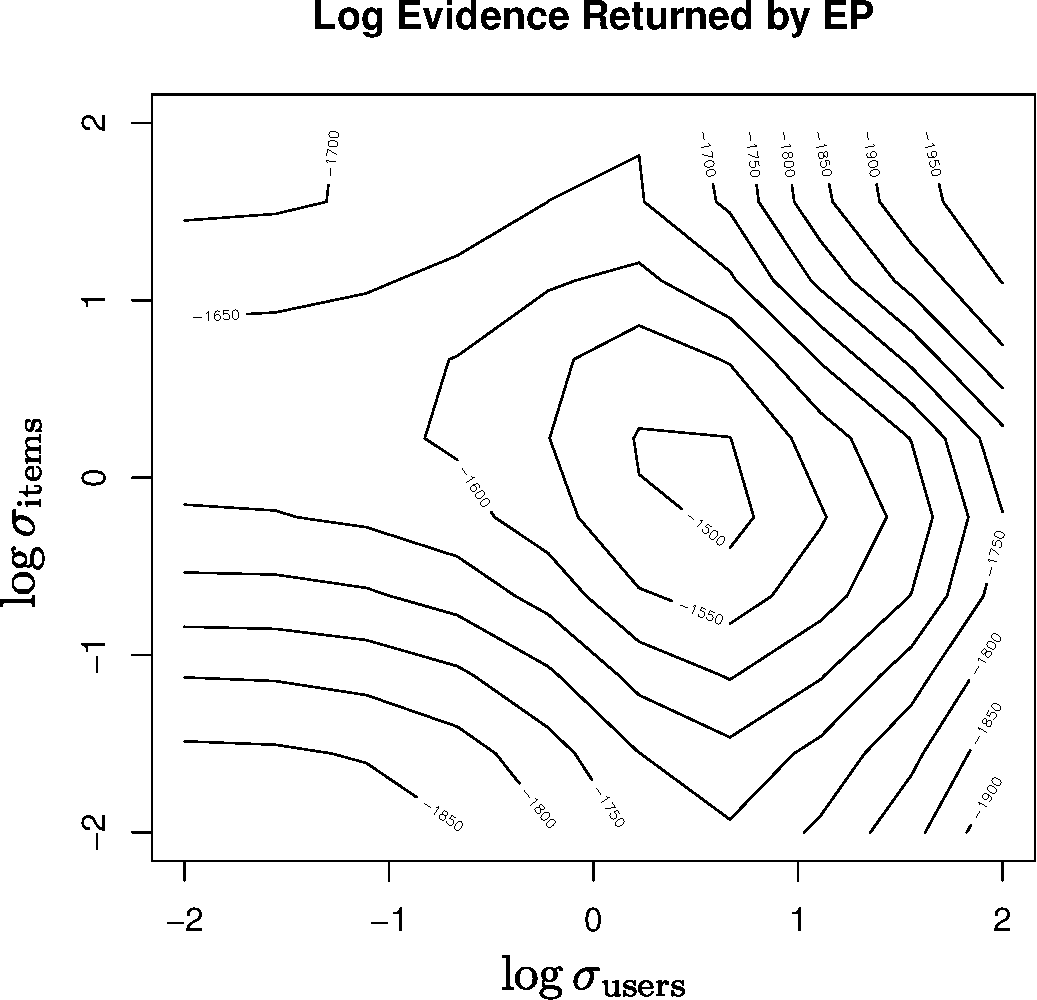
\includegraphics[scale=0.4]{figs/plotEvidence.pdf}
\caption{Logarithm of the evidence returned by EP when run on the first training set of the experiments with synthetic data.
Different values are considered for the lengthscale parameters $\sigma_\text{users}$ and $\sigma_\text{items}$.
The synthetic data are generated using $\log \sigma_\text{users} = 0$ and $\log \sigma_\text{items} = 0$.
The highest evidence returned by EP corresponds to values of $\log \sigma_\text{users}$ and
$\log \sigma_\text{items}$ close to zero.}\label{fig:experimentEvidence}
\end{figure}

Before the main experiments we perform an initial investigation to show that approximation of the model evidence given by EP can be used to
tune the kernel hyper-parameters in the proposed multi-user model. For this, we use the synthetic dataset
described in the main document. Figure \ref{fig:experimentEvidence} shows a contour plot of the log-evidence returned by EP 
when run on the first training set of the experiments with synthetic data and 100 users.
Different values are considered for the lengthscale parameters $\sigma_\text{users}$ and $\sigma_\text{items}$.
The synthetic data are generated using $\log \sigma_\text{users} = 0$ and $\log \sigma_\text{items} = 0$.
The highest evidence returned by EP corresponds to values of $\log \sigma_\text{users}$ and $\log \sigma_\text{items}$ close to zero.
In this experiment we are running EP using a total of 20 latent functions,
while the data are generated using only 5 latent functions.
As mentioned in the main document, the proposed multi-user model
seems to be robust to over-fitting and over-estimation of
the number of latent functions does not seem to harm predictive performance.

\subsection{Comparison with other multi-user methods}

\paragraph{Alternative models.} Two versions of the proposed collaborative preference (CP) model are used.
The first version (CPU) takes into account the available user features, as described in Section \ref{sec:model}. The second version (CP) ignores these features by
replacing $\mathbf{K}_\text{users}$ in (\ref{eq:priorW}) with the identity matrix.
We compare to the two multi-user methods described in Section \ref{sec:relatedWork}. 
We denote to the model of Birlutiu \emph{et al.} as (BI), and that of
Bonilla \emph{et al.} as (BO).
We implement BO and BI using the preference kernel and EP for approximate inference.
Remember, that BI does not incorporate user features, and BO must include them.
Finally, we consider a single user approach (SU) which fits a different GP classifier independently to the data of each user.

\paragraph{Experimental procedure.} Due to the high computational cost of BI and BO, to compare to these methods we must subsample the datasets, keeping only 100 users.
The available data were split randomly into training and test sets of item pairs,
where the training sets contain 20 pairs per user in Sushi, MovieLens and Election, 15 pairs in Jura and
30 in Synthetic. This was repeated 25 times to obtain statistically meaningful results.
In CPU and CP, we selected the number of latent functions $D$ to be $20$ (see Table \ref{tab:small}).
In general, the proposed models, CPU and CP, are robust to over-fitting and over-estimation of
$D$ does not harm predictive performance. Note that the Synthetic dataset is generated
using $D=5$ and CPU and CP still obtain very good results using $D = 20$.
This automatic pruning of unnecessary degrees of freedom seems to be common
in methods based on variational Bayes \cite{MacKay2001}.
We selected the kernel lengthscales to be equal to
the median distance between feature vectors. This leads to good empirical performance
for most methods. An exception is BO, where the kernel hyperparameters
are tuned to some held-out data using automatic relevance determination.
In our model, we can also estimate the kernel
lengthscales by maximizing the EP approximation of the model evidence,
as illustrated in the Supplementary material. This alternative approach can be used
when it is necessary to fine tune the lengthscale parameters to the data. In CPU we use $U_0 = 25$ pseudo inputs for approximating $\mathbf{K}_\text{users}$.
These pseudo inputs are selected randomly from the set of available data points.
Similarly, in CP and CPU, we use $P_0 = 25$ pseudo inputs for approximating $\mathbf{K}_\text{items}$,
except in the Jura and Election datasets (which contain fewer items) where we use $P_0 = 15$.
The results obtained are not sensitive to the number of pseudo inputs used, as long as
the number is not excessively low.

%\renewcommand{\arraystretch}{0.9}
\newcommand{\ic}{\hspace{0.25cm}}
\begin{table}
\begin{minipage}[b]{0.49\columnwidth}
\centering
\caption{Average test error with 100 users.}
\resizebox{0.9 \columnwidth}{!}{
\begin{tabular}{@{\ic}l@{\ic}c@{\ic}c@{\ic}c@{\ic}c@{\ic}c@{\ic}c@{\ic}}
\hline
\textbf{Dataset} &\textbf{CPU}&\textbf{CP}&\textbf{BI}&\textbf{BO}&\textbf{SU}\\
\hline
Synthetic&0.162&0.180&0.175&\bf{0.157}&0.226\\
Sushi&0.171&0.163&\bf{0.160}&0.266&0.187\\
MovieLens&0.182&\bf{0.166}&0.168&0.302&0.217\\
Election&0.199&0.123&\bf{0.077}&0.401&0.300\\
Jura&0.159&\bf{0.153}&\bf{0.153}&0.254&0.181\\
\hline
\end{tabular} \label{tab:errorSmallDatasets}
}
\end{minipage}
\begin{minipage}[b]{0.5\columnwidth}
\centering
\caption{Training times (s) with 100 users.}
\resizebox{0.9 \columnwidth}{!}{
\begin{tabular}{@{\ic}l@{\ic}r@{\ic}r@{\ic}r@{\ic}r@{\ic}r@{\ic}r@{\ic}}
\hline
\textbf{Dataset} &\textbf{CPU}&\textbf{CP}&\textbf{BI}&\textbf{BO}&\textbf{SU}\\
\hline
Synthetic&7.793&9.498&22.524&311.574&0.927\\
Sushi&5.694&4.307&20.028&215.136&0.817\\
MovieLens&5.313&4.013&19.366&69.048&0.604\\
Election&13.134&12.408&20.880&120.011&0.888\\
Jura&3.762&2.404&15.234&88.502&0.628\\
\hline
\end{tabular} \label{tab:timeSmallDatasets}
}
\end{minipage}
\label{tab:small}
\end{table}



\paragraph{Results.} Average test errors are shown in Table \ref{tab:errorSmallDatasets}. 
Those highlighted in bold are statistically different to those not highlighted
(calculated using a paired $t$ test). Overall, CP and CPU outperform SU and BO, and breaks even with BI;
the final result is notable as BI learns the full mean and covariance structure across all users,
ours uses only a few latent dimensions, which provides the key to scaling to many more users.
CP outperforms CPU in all cases except in the Synthetic dataset. In the real-world datasets, users with 
similar features do not seem to have similar preferences and so correlating behavior of users with similar features is detrimental.
In this case, the unsupervised learning of similarities in user preferences is more useful for prediction than the user features.
This also explains the poor overall results obtained by BO.
Finally, running times in seconds are presented in Table \ref{tab:timeSmallDatasets}. 
The entries for BO do not include the time spent by this method to tune the kernel hyper-parameters.
CP and CPU are faster than BO and BI. The FITC approximation imposes
a large multiplicative constant in the cost of CP and CPU so for larger datasets the gains are much larger.

\subsection{Active learning on large datasets}

\renewcommand{\ic}{\hspace{0.3cm}}
\begin{table}
\centering
\caption{Test error for each method and active learning strategy with at most 1000 users. Standard deviations ommitted for readability.}
\resizebox{0.95\textwidth}{!}{
\begin{tabular}{@{\ic}l@{\ic}@{\ic}c@{\ic}c@{\ic}c@{\ic}@{\ic}c@{\ic}c@{\ic}c@{\ic}@{\ic}c@{\ic}c@{\ic}c@{\ic}}
\hline
\textbf{Dataset}&\textbf{CPU-B}&\textbf{CPU-E}&\textbf{CPU-R}&
\textbf{CP-B}&\textbf{CP-E}&\textbf{CP-R}&\textbf{SU-B}&\textbf{SU-E}&\textbf{SU-R}\\\hline
Synthetic&\underline{\bf{0.136}}&\bf\underline{{0.136}}&0.14&\bf{0.154}&0.161&0.179&\bf{0.253}&0.263&0.276\\
Sushi&\bf{0.150}&0.155&0.185&\underline{\bf{0.143}}&0.151&0.179&\bf{0.183}&0.199&0.215\\
MovieLens&\bf{0.172}&0.177&0.200&\underline{\bf{0.165}}&0.171&0.196&\bf{0.233}&0.24&0.253\\
Election&0.221&\bf{0.188}&0.265&\underline{\bf{0.107}}&\underline{\bf{0.103}}&0.184&\bf{0.331}&0.349&0.344\\
Jura&\bf{0.143}&\bf{0.144}&0.17&\underline{\bf{0.138}}&\underline{\bf{0.138}}&0.17&0.183&\bf{0.169}&0.201\\
\hline
\end{tabular}
}
\label{tab:large}
\end{table}


\begin{figure}[h!]
\centering
\resizebox{\textwidth}{!}{
\begin{tabular}{ccc}
Synthetic&
Sushi&
MovieLens\\
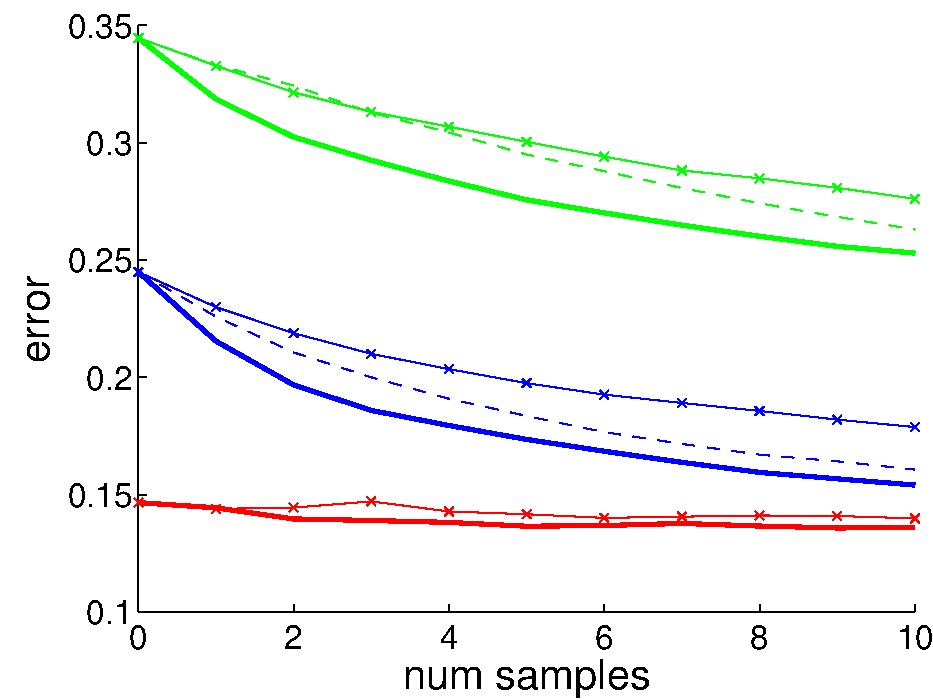
\includegraphics[scale=0.3]{figs/error_syntheticDataLargeScale.pdf}&
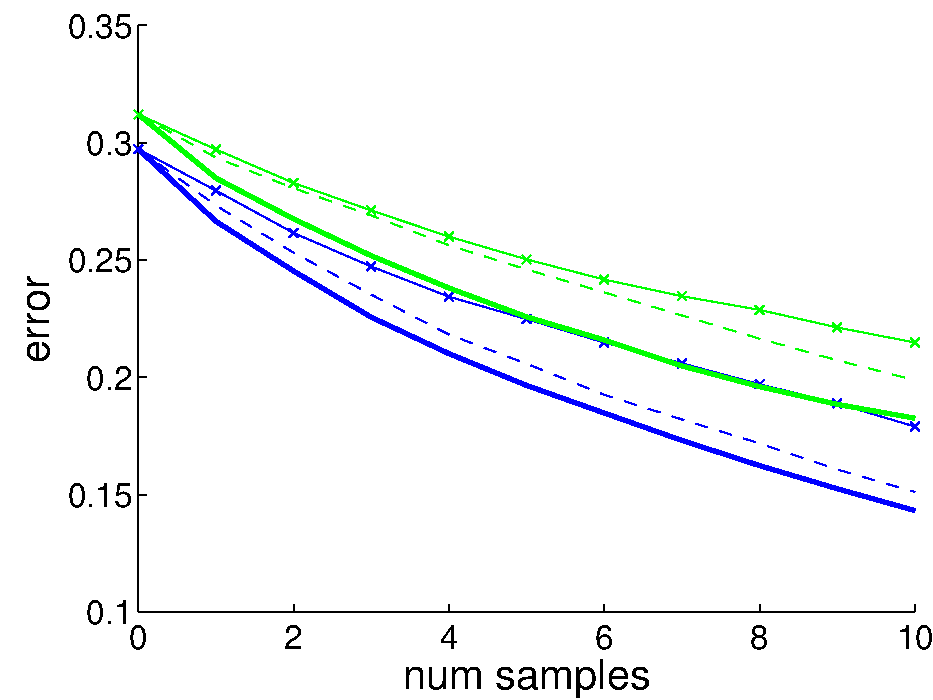
\includegraphics[scale=0.3]{figs/error_sushiDataLargeScale.pdf}&
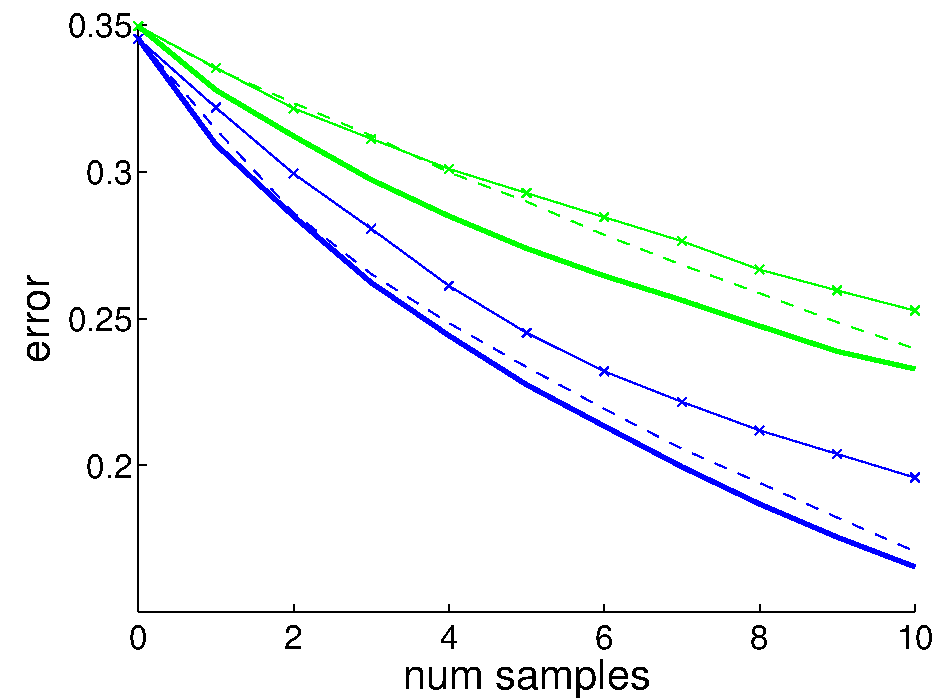
\includegraphics[scale=0.3]{figs/error_movieLensDataLargeScale.pdf}\\
Election&
Jura&
\\
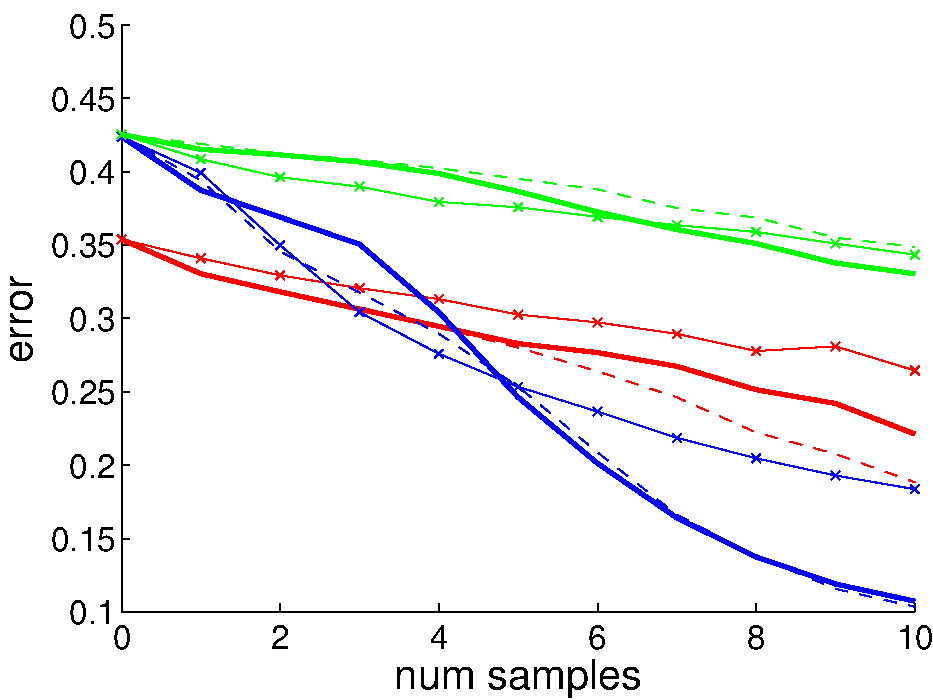
\includegraphics[scale=0.3]{figs/error_electionDataLargeScale.pdf}&
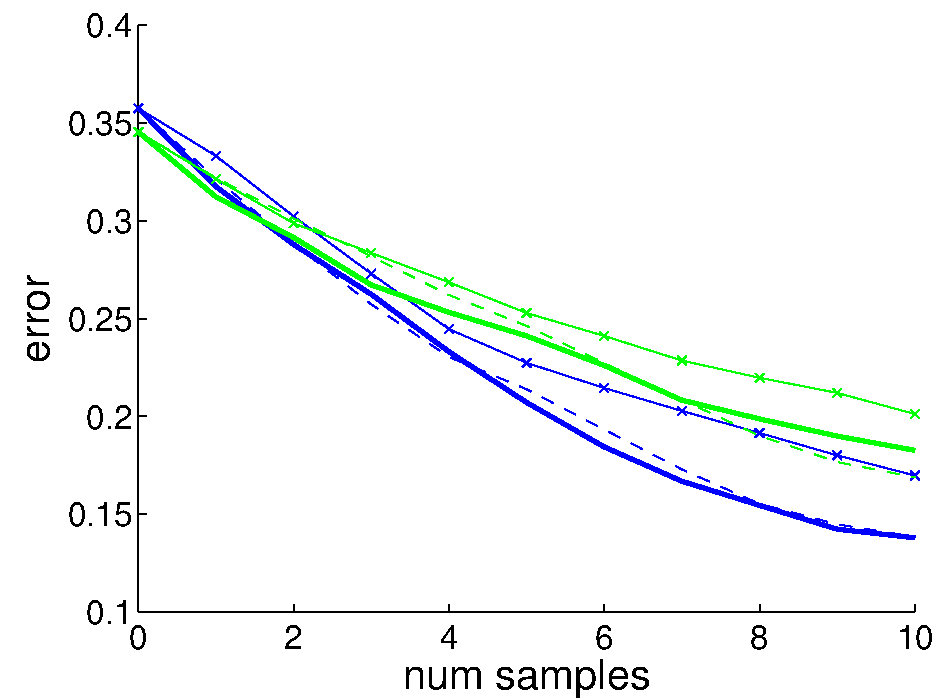
\includegraphics[scale=0.3]{figs/error_juraDataLargeScale.pdf}&
\hskip0.6cm \raisebox{0.08\height}{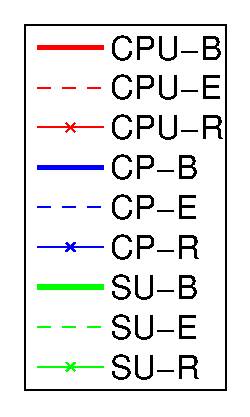
\includegraphics[scale=0.45]{figs/legend.pdf}}
\end{tabular}
}
\caption{Average test error for CPU, CP and SU, using the strategies BALD (-B), entropy (-E) and random (-R) for active learning.
For visual clarity, the curves for CPU are included only in the Synthetic and Election datasets.}
\label{fig:learningcurves}
\end{figure}

Here we evaluate the performance of BALD,
in particular, we compare CPU, CP, and SU using BALD (-B), Maximum Entropy Sampling (-E) and random sampling (-R).
We now use all the available users from each dataset, with a maximum of 1000 users.
For each user the available preference data are
split randomly into training, pool and test sets with 5, 35 and 5 data points respectively
in Synthetic, Sushi and MovieLens, 3, 22 and 3 data points in Election
and 3, 15 and 3 data points in Jura.
Each method is fitted using the training sets and its performance
is then evaluated on the corresponding test sets. After this,
the most informative data point is identified in each
of the pool sets. These data points are moved into the corresponding training sets
and the process repeats until 10 of these active
additions to the training sets have been completed.
The entire process, including the dataset splitting is repeated 25 times. 
Figure \ref{fig:learningcurves} shows the learning curve for each method.
For clarity, the curve for CPU is included only for the Synthetic and Election datasets; in the other datasets CPU is marginally outperformed by CP.
Average errors after 10 queries from the pool set of each user are summarized in Table \ref{tab:large}.
For each model (CPU, CP and SU), the results of the best active learning strategy are highlighted in bold.
The results of the best model/active learning strategy combination are underlined.
Highlighted results are statistically significant with respect to non-highlighted
results according to a paired $t$ test.
BALD always outperforms random sampling and usually outperforms or obtains equivalent performance to MES. 
In particular, BALD significantly outperforms MES in nine cases,
while MES is better than BALD in only two cases.

\section{Conclusions\label{sec:conclusions}}

We have proposed a multi-user model that combines collaborative filtering methods
with GP binary preference modeling.
We have shown that the task of learning user preferences can be recast as a particular case of binary classification with GPs
when a covariance function called the preference kernel is used.
We have also presented BALD,
a novel active learning strategy for binary classification models with GPs. The proposed multi-user model with BALD performs favorably on simulated and real-world data against single-user methods
and existing approaches for multi-user preference learning, whilst having significantly lower computational times than competing multi-user methods.


{
\bibliographystyle{apalike}
\bibliography{bib/bibliog}
}

\newpage

\end{document}
